\documentclass[12pt]{report}

% Page layout
\usepackage[a4paper, margin=3cm]{geometry}

%Hyperlink
\usepackage{hyperref}
%\usepackage[hidelinks]{hyperref}

% Font and text formatting
\usepackage{setspace}
\usepackage{graphicx}
\usepackage{amsmath}
\usepackage{amsfonts}
\usepackage{amssymb}
\usepackage{subcaption}
\usepackage{tabularx}
\usepackage{algorithm}
\usepackage{algpseudocode}
\usepackage{float}
\usepackage{multirow} % for multirow cells
\usepackage{array}   % for more flexible column definitions
\usepackage{tocbibind} 
\usepackage{acronym}
% Font setup
%\usepackage{fontspec}
%\setmainfont{Calibri}
\usepackage{enumitem}
\setlist{leftmargin=5.5mm}
\newlist{myitemize}{itemize}{3}
\setlist[myitemize,1]{label=\textbullet,leftmargin=1.5cm}

% Custom command for cover (thesis title page)
\newcommand{\cover}[4]{
    \begin{titlepage}
        \centering
        \vspace*{2cm}
        \Huge\textbf{#1}\\
        \vspace{1.5cm}
        \Large\textbf{By}\\
        \vspace{0.5cm}
        \Large\textbf{#2}\\
        \vspace{3cm}
        \Large\textbf{Advisor: #3}\\
        \vspace{0.5cm}
        \Large\textbf{Co-advisor: #4}\\
        \vfill
    \end{titlepage}
}

% Table formatting
\usepackage{array}
\renewcommand{\arraystretch}{1.5}

% Paragraph formatting
% \setlength{\parindent}{0pt}
\setlength{\parskip}{0.75\baselineskip}

% Section and subsection formatting
\usepackage{titlesec}
\titleformat{\chapter}[display]{\centering\normalfont\fontsize{14}{15}\bfseries}{\MakeUppercase{\chaptertitlename} \thechapter}{0em}{\MakeUppercase}
\titlespacing*{\chapter}{0pt}{-50pt}{4em}

\titleformat{\section}{\normalfont\fontsize{14}{15}\bfseries}{\thesection}{1em}{}
\titlespacing*{\section}{0pt}{1em}{0em}

\titleformat{\subsection}{\normalfont\fontsize{12}{14}\bfseries}{\thesubsection}{1em}{}
\titlespacing*{\subsection}{0pt}{1em}{0em}

% Page numbering
\usepackage{fancyhdr}
\pagestyle{fancy}
\fancyhf{}
\fancyhead[L]{\textcolor{gray!80}{\scriptsize{\uppercase{Risk Informed UAV Pathfinding, UPX}}}}
\fancyfoot[C]{\thepage}
\fancyfoot[C]{{\textcolor{gray!80}{\footnotesize\textbf{\thepage/\pageref{LastPage}}}}}
\renewcommand{\headrulewidth}{0.4pt}
\renewcommand{\chaptermark}[1]{\markboth{#1}{}}

\usepackage{xcolor}
\usepackage{lastpage}

% Bibliography
\usepackage{csquotes}
\usepackage[backend=biber, style=apa,]{biblatex}
\addbibresource{UPXNEW.bib}

\begin{document}
    %------------------- TITLE COVER-----------------------
     \begin{titlepage}
        \begin{center}
            \textbf{\LARGE Development of Risk-Informed UAV Pathfinder Based on A* Algorithm}
    
            \vspace{0.5cm}
            
                
            \textbf{\Large Micko Lesmana}
            \vspace{0.5cm}

            \textbf{\Large 11201901010}
            \vspace{3.5cm}  

            
\includegraphics[width=0.4\textwidth]{General Image/IULISymbol.PNG}
            \vspace{3.5cm}


            \large Undergraduated Thesis\\
                
            \vspace{0.8cm}
                
            Department of Aviation Engineering\\
            International University Liaison Indonesia\\
            BSD City\\
            7 July 2024
                
        \end{center}
    \end{titlepage}
    %------------------- APPROVAL PAGE---------------------

        \begin{center}
            \textbf{\Large Approval Page}
            \vspace{0.4cm}

            \textbf{\Large Report}
            \vspace{0.4cm}
            
            \textbf{\Large Risk Informed UAV Pathfinding, UPX}
            \vspace{0.4cm}

            \textbf{\large 3 December 2022}
            \vspace{1cm}
            
                
            \textbf{\large Micko Lesmana}
            \vspace{0.3cm}

            \textbf{\large 11201901010}
            \vspace{0.3cm}
                
            \textbf{\large Department of Aviation Engineering}
            \vspace{2cm}

            \textbf{\large Acknowledge by:}
            \vspace{3cm}

        %\begin{tabular}{@{}p{2.5in}p{2.5in}@{}}
        
        %Company Surpervisor:                & Head of Department\\
        %Date:                               & Aviation Engineering:\\
                                            %& Date:\\
%%                                            & \centerline{\includegraphics[width=0.1\textwidth]{IULIstamp}}\\
        %\rule{5cm}{0.5pt}                   & \rule{5cm}{0.5pt}\\
        %\end{tabular}
    \end{center}
    %-----------------------------------:TABLE OF CONTENT--------
    \tableofcontents
    \listoffigures
    \listoftables
   
    \newpage
    \chapter*{LIST OF ACRONYMS}
    \addcontentsline{toc}{chapter}{List of Abbreviations}
    \begin{acronym}[geoJSON]
        \acro{A*}{A-star}
        \acro{AIS}{Abbreviated Injury Scale}
        \acro{API}{Application Programming Interface}
        \acro{BBN}{Bayesian Belief Networks}
        \acro{BC}{Blunt Criteria}
        \acro{CFIT}{Controlled Flight Into Terrain}
        \acro{CRS}{Coordinate Reference System}
        \acro{DOJC}{Dropped or Jettisoned Component}
        \acro{DoD}{United States Department of Defense}
        \acro{ETA}{Event Tree Analysis}
        \acro{FAA}{Federal Aviation Administration}
        \acro{FMECA}{Failure Mode, Effects and Criticality Analysis}
        \acro{FTA}{Fault Tree Analysis}
        \acro{GHSL}{Global Human Settlement Layer}
        \acro{GIS}{Geographic Information System}
        \acro{GPS}{Global Positioning System}
        \acro{GRM}{Ground Risk Model}
        \acro{geoJSON}{Geographic JavaScript Object Notation}
        \acro{ICAO}{International Civil Aviation Organization}
        \acro{KE}{Kinetic Energy}
        \acro{LOC}{Lost of Control}
        \acro{MTBF}{Mean Time Between Failure}
        \acro{OSM}{OpenStreetMap}
        \acro{PDF}{Probability Density Function}
        \acro{RRT}{Rapidly Exploring Random Tree}
        \acro{UDS}{Unpremediated Descent Scenario}
        \acro{UAS}{Unmanned Aerial System}
        \acro{UAV}{Unmanned Aerial Vehicle}
        \acro{UPX}{UAV Pathfinding eXtension}
        \acro{CE}{Casualty Expectation}
        \acro{AGL}{Above Ground Level}
        \acro{BFS}{Bread-First Search}
        \acro{DFS}{Depth-First Search}
        \acro{ACO}{Ant Colony Optimization}
        \acro{RRT}{Rapidly-Exploring Random Tree}
    \end{acronym}
    \newpage
    


%---------------------------------------CHAPTER 1-------------------------------------

%s/\[1\]/\cite{washington_review_2017}/g
%s/\[4\]/\cite{breunig_modeling_2018}/g
%s/\[5\]/\cite{pat-cornell_uncertainties_1996}/g
%s/\[6\]/\cite{primatesta_ground_2020}/g
%s/\[7\]/\cite{kim_risk-based_2022}/g
%s/\[8\]/\cite{weibel_safety_2012}/g
%s/\[9\]/\cite{burke_system-level_2011}/g
%s/\[10\]/\cite{ball_crash_2012}/g
%s/\[11\]/\cite{primatesta_ground_2020}/g
%s/\[12\]/\cite{wu_development_2012}/g
%s/\[13\]/\cite{melnyk_third-party_2014}/g
%s/\[14\]/\cite{ale_assessment_2000}/g
%s/\[15\]/\cite{shelley_model_2016}/g
%s/\[16\]/\cite{bleier_risk_2015}/g
%s/\[17\]/\cite{small_aviation_2009}/g
%s/\[18\]/\cite{dalamagkidis_evaluating_2008}/g
%s/\[19\]/\cite{klepeis_national_2001}/g
%s/\[20\]/\cite{clothier_casualty_2007}/g
%s/\[21\]/\cite{harwick_approved_2007}/g
%s/\[22\]/\cite{magister_small_2010}/g
%s/\[23\]/\cite{noauthor_openstreetmap_2022}/g
%s/\[24\]/\cite{noauthor_global_2023}/g
%s/\[25\]/\cite{noauthor_unmanned_2015}/g
%s/\[26\]/\cite{cour-harbo_ground_2020}/g
%s/\[27\]/\cite{la_cour-harbo_quantifying_2019}/g
%s/\[28\]/\cite{aalmoes_conceptual_2015}/g
%s/\[29\]/\cite{cole_hazards_1997}/g
%s/\[30\]/\cite{cole_hazards_1997}/g
%s/\[31\]/\cite{gonzales_faas_2017}/g
%s/\[32\]/\cite{primatesta_risk-aware_2019}/g

\chapter{Introduction}
    \section{Introduction}
        \ac{UAV} also known as a drone, is getting more recognition in recent years. The booming of UAV is caused by the
	    component needed to manufacture the UAV, especially microcontrollers getting cheaper, and smaller
	    \cite{austin_4_2024}. Compare to previous UAV iteration, UAV nowadays offers much wider capability, such as
	    enhanced range, the ability to mount hardware, and camera for example, and of course easily deployable without
	    requiring many technicians to maintain them.

		    UAV are often being used in area where it is dangerous, impractical, and expensive for human. The affordable
	    entry point of using a UAV incentivized emerging industries to exploit the capability that UAV offer. Not only
	    that but the existing industry is also getting interested to use UAV as an augmentation to its existing
	    operational infrastructure. And that industries are, logistics companies, agricultural companies, multimedia
	    companies, and surveyors to name a few \cite{dji_dji_2023}.

            Although it provides a great solution, UAV have the potential to pose risks to people, property, and other
        aircraft. Many countries have regulations in place that require UAV to be operated in a safe and responsible
        manner \cite{faa_ecfr_2016}. Risk-based UAV path planner can help to ensure that UAV are operated safely and
        responsibly. By considering potential risks and hazards, a risk-based approach can help to reduce the likelihood
        of accidents or incidents occurring during the flight. By considering potential risks and hazards, this approach
        can help to reduce the likelihood of accidents or incidents occurring during deployment.

            Other than its impacts towards public, UAV can also potentially impact the environment, for example by
        disturbing wildlife or damaging natural habitats \cite{holland_how_2015}. UAV path planner can help to minimize
        these impacts by establishing rules around the use of UAV in sensitive areas.
    \section{Research purpose}
        For ensuring the safety and efficiency of UAV operations, this research aims to develop a
        UAV trajectory planning based on the risk assessment on the ground.
    \section{Research scope}
        \begin{myitemize}   
            \item UAV model that being used in this research are fixed wing and multirotor.
            \item This research only use point mass representation with generalize aerodynamic equation.
            \item Based on the point above, UAV failure is assumed to be only power failure, without damage to its shape.
            \item Risk assessed in this paper are combination of human exposed area and area that can cause major accident such as airfields, and power station.
            \item This research use Jakarta, Indonesia as its geographic location, since it has varying building density, rivers, and randoml patch of lands.
        \end{myitemize}
        
    \section{Research problem}
        \begin{myitemize}
            \item There are risks associated when of UAV falls on the ground.
            \item Modeling physical interaction of UAV crash.
            \item Selection of pathfinding algorithm to get optimum time.
        \end{myitemize}
        
    \section{Significance of the study}
        UAV Pathfinder application could be one of the toolkit for UAV operator to plan their safe operation of
        flying their UAV, reducing inccident and accident. Developer and researcher could use the library itself as an
        extension or starting point in the development of the \ac{UAS} Traffic Management application.
        
    \section{Research question}
        \begin{myitemize}
            \item Which kind of geographic data and data processing model perfectly suited for pathfinding risk assesment.  
            \item How to statistically create the best approximation of crash dynamics.
            \item What kind of pathfinding method that produces the quasi-optimal path without sacrificing computational time.
        \end{myitemize}

    \section{Thesis Structure}


%---------------------------------------CHAPTER 2-------------------------------------
\chapter{Literature Review}
    \section{Overview}
        In this part of the literature review, we will discuss two main concepts: the Ground Risk Model and the Path
        Finder. in the first part , we will examine the Ground Risk Model, which involves discussing the concept of
        probability within a spatial context. Consider this scenario: if we want to calculate the likelihood of someone
        being hit by a drone in a specific location, how do we model this phenomenon? As you can see, scenarios like
        this are key to understanding the Ground Risk Model.

        Next, we will explore the Path Finder. After identifying a model that answers the question of where a UAV is
        most likely to hit someone, we move on to the next question: how do we navigate the UAV or provide the safest
        route to minimize the risk of severe casualties? This is why we will discuss the Risk-Based Path Finder.
    
    \section{Ground risk model}
        A ground risk model is a type of assessment tool that is used to evaluate the potential risks associated with
        the operation of UAV. This model takes into account a variety of factors, including the physical environment in
        which the UAV will be operating, the capabilities, and the limitations of the UAV itself. The goal of a ground
        risk model is to identify and prioritize potential risks in order to produce inform decision-making and risk
        management strategies for UAV operations.

        We found a total of 22 different research papers that contributed to our study on ground risk models. Various
        approaches have been taken to develop ground risk models for UAVs. One approach is the use of scenario-based
        methods, as discussed in the research of \cite{ancel_real-time_2017}, which involves the development of detailed
        scenarios that describe potential UAV operations and the associated risks.
            
        To clarify further, in the research done by \cite{ancel_real-time_2017}, there are two common methods for
        describing the severity of accidents using scenario-based approaches. These scenarios are typically coupled with
        safety and hazard levels on a per-operation basis. The first method utilizes a lookup table to determine the
        severity of an accident. The second method represents the scenario as a directed acyclic graph, a type of tree
        graph, where we start at the root node and traverse based on yes or no questions. These questions can range from
        simple ones, such as whether the UAV hit a person, to more detailed ones, such as whether the accident caused
        harm.
            
        This method is computed using techniques such as risk tree diagrams, Bayesian belief networks
        \cite{ancel_real-time_2017}, and hazard risk assessment matrices \cite{barr_preliminary_2017}. Although these
        methods might produce different analyses, they generally describe the same phenomena.
            
        From the description above, it appears that scenario-based models do not suit our needs for a spatially based
        ground risk model. Essentially, they reduce to questions of general progression from the point of impact to the
        accident caused by the drone. They provide no information on how the position of the UAV affects the casualty
        risk of failed operations and only serve as a preliminary assessment.
            
        To add a spatial component to our models, we can simply incorporate location information into the yes/no
        question tree graph. What I mean by this is to propose an idea where, in a certain area, if a UAV somehow falls,
        does it cause harm, and based on the surrounding environment, does that harm result in fatality?
            
        This brings us to the most widely used method, so called ground probabilistic risk assessment methods, which
        involve the quantification of risks per area using probability and consequence metrics. Although a greater
        number of research papers use this method, as compiled by \cite{washington_review_2017}, our concept shown in
        figure \ref{fig:prime_example} is derived from the research conducted by \cite{primatesta_ground_2020}. 

        \begin{figure}[H]
            \centering
            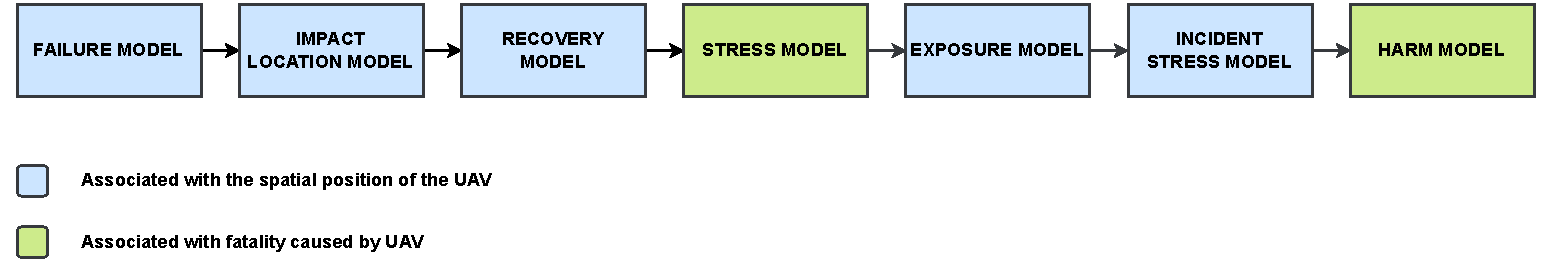
\includegraphics[width=\textwidth]{General Image/OSM Drone-GROUND.pdf}
            \caption{Components of ground risk model adopted from \protect\cite{primatesta_ground_2020}}
            \label{fig:prime_example}
        \end{figure}

        A ground probabilistic risk assessment model, shortened to ground risk model, of a UAV typically consists of
        several subcomponents that are used to assess various factors that can impact the safety and effectiveness of
        UAV operations. These components in the ground risk model include the failure model, impact location model,
        recovery model, stress model, exposure model, incident stress model, and harm model, which will be explained
        further below.

        However, since this is the most widely used approach, it is not surprising that this approach is not new, as
        many earlier researchers have already followed guidelines to model these components. For example,
        \cite{breunig_modeling_2018} provides a general model guideline. These guidelines focus more or less on the
        probability of said accidents causing fatalities but do not compute the overall area risk.
            
        \cite{washington_review_2017} offers a meta-analysis of different kinds of research using more or less the same
        paradigm to describe the ground risk model. \cite{washington_review_2017} itself uses the method of its analysis
        based on the guidelines from \cite{pat-cornell_uncertainties_1996}, which studied the level of analytical detail
        when modeling risk. \cite{pat-cornell_uncertainties_1996} provides us with a degree of certainty ranging from
        one to six, where one uses a very simple model and six accounts for every possible situation that can affect the
        model.
            
        After a thorough discussion, we derived our study based on \cite{primatesta_ground_2020} simply because it shows
        the most comprehensive way to calculate the ground risk model, which can be summarized into Equation
        \ref{eq:general_probability}.
        
        \begin{equation}\label{eq:general_probability}
            P_{fatal}(x) = P_{failure}(x) \cdot P_{impact}(x) \cdot P_{recovery} \cdot P_{stress} \cdot P_{exposure}(x) \cdot P_{incident}(x) \cdot P_{harm}(x)
        \end{equation}
        
        All of these models are represented as the probability of the said event-model occurring. Where \(P\) is a
        probability of an event and \(x\) is the location on a grid map. If we take a closer look at Equation
        \ref{eq:general_probability}, some \(P_n\) terms do not contain any location parameter. This is because those
        probabilities are applied as global variables to every area. 
        
        Back to the model, since all models occur consecutively from the failure model to the harm model, each component
        of the ground risk model is multiplied by the others. Although many papers do not use all of these components in
        their ground risk models and often use different methodologies to analyze the same component, the fundamental
        approach remains consistent. For example, \cite{primatesta_ground_2020} only use the event, impact location, and
        fatality models, while \cite{kim_risk-based_2022} use the event, impact, exposure, incident stress, and harm
        models. Despite apparent differences in modeling ground risk, researchers sometimes combine multiple
        subcomponents into one. For instance, in \cite{primatesta_ground_2020}, the fatality model component is, in
        fact, a combination of the incident, stress, and harm models. All the models in ground risk assessment are
        explained in following sub-chapters.

        \subsection{Failure model}
            A failure model is the first subcomponent in the ground risk model that evaluates the potential for failures
            in UAV. This potentially leads to a crash impact in a given variety of factors that can contribute to UAV
            failures, including design and manufacturing defects, operational errors, and environmental factors.

                The failure model can help to understand on how the UAV would behave after experiencing the failure,
            \cite{washington_review_2017} described four distinct events following the failure. Which are \ac{UDS}, 
            \ac{LOC}, \ac{CFIT}, and \ac{DOJC}.

            All of these failure events describe how the UAV crashes into the ground. UDS is a mode where the drone
            automatically enters a safe mode and tries to land as safely as possible. Drone manufacturers often
            implement this feature when critical components are detected to be defective. UDS can also be triggered when
            the UAV loses its signal to its pilot. Most mid- and high-priced drones usually have this feature, such as
            those from \cite{dji_consumer_2024}.
                
            Controlled flight into terrain occurs when the UAV still has flight authority, but its main propulsion is no
            longer working or its battery is at very low power, allowing it to only move its control surface servos. It
            is similar to UDS, except that in UDS, the UAV still has propulsion power. Also like UDS, if the UAV is
            advanced enough \cite{nemire_dji_2015}, it can auto-navigate to a safer area.
                
            Loss of control scenario occurs when the UAV is no longer responsive and has lost its navigation system,
            causing it to fly away while maintaining its velocity and altitude until it runs out of energy or crashes
            into terrain. This condition is much more degraded compared to UDS. Lastly, the "dropped or jettisoned"
            scenario, probably the least common failure stated by \cite{washington_review_2017}, occurs when some
            components detach from the drone and fall to the ground.

            Although the definition of a ways that UAV can fell into the terrain, it does not necessarly help us
            calculate the likelihoodness of a UAV to fell into the ground. With that being said this definition can help
            us to formulate the descent model of the ground risk model.
            
            If we want to calculate the probability of the drone starts to fail, there are two main models that we can
            use. The first one is  failure model proposed by \cite{breunig_modeling_2018} and \cite{weibel_safety_2012}
            where it is based on historical data. Data driven historical data are using previous UAV crash, and its UAV
            specification as a starting point for data interpolation and extrapolation for calculating so called
            \ac{MTBF}.

            Unfortunately since UAV industries is in its infancy and an added fact with many variants of UAV already
            exist in short period of time. There are not enough historical data to make an interpolation, which is an
            issue commented by \cite{breunig_modeling_2018}, many model using an MTBF simply use a standard assumed by
            \cite{arc_unmanned_2015} which is average of 1 failure per 100 hours of flight for small UAV.

            Although with its limitation, there are few research that trying to emulate MTBF to solve target level of
            safety to help certifying authorities to make a propper judgment in regards to ever growing small UAV
            industry. Such model is developed by \cite{burke_system-level_2011}, where they make a system-level
            airworthiness tools that predict how safe a UAV is based on the sizes of the aircraft which is explained the
            equation \ref{eq:mtbf} below.

            \begin{equation}\label{eq:mtbf}
                MTBF = \frac{\rho \pi b^2}{2.78} = k(\rho \pi b^2)
            \end{equation}

            Where \(\rho\) is population density, \(b\) is geometric wingspan of the drone, and \(k\) is population
            correction factor, where k is \(\frac{1}{2.78}\) in a setting where the population density is calculated per
            square miles. This equation is derived from target level safety algorithm proposed by
            \cite{burke_system-level_2011}. Which then derived from \ac{CE} equation \ref{eq:CE}

            \begin{equation}\label{eq:CE}
                CE = P_f \times P_d \times A_l \times P_k \times {S}
            \end{equation}

            Where \(CE\) is expected casualty rate per flight hours, \(P_f\) is the probability of failure in failure
            per flight hour, \(P_d\) is the population density in people per square mile, \(A_l\) is the dimensionless
            lethal area, \(P_k\) is fatality probability, and \(S\) is the dimensionless shelter factor. We then change
            the \(P_d\) as a \(\rho\) to signified the average in time for population in a given mission area. \(A_l\)
            is modeled from using the maximum circular area of the UAV itself which is the maximum wing span \(b\) in
            feet or in the case of multirotor, maximum diagonal distance. Therefore \(A_l\) can be substitute into \(\pi
            b^2\). Pointer given by \cite{burke_system-level_2011} simply using \(A_l\), which calculate in feet, will
            give an error when being multiplied by \(\rho\) where it is in square miles. Therefore
            \cite{burke_system-level_2011} give an error correction to divide \(\rho\) with the number of 1 \(ft^2\) in
            a 1 \(mile^2\) which roughly is 27.8 million. 

            \cite{burke_system-level_2011} normalized the \(P_k\) to 1 to argue based on the fact provided by
            \cite{arc_unmanned_2015}. This normalization came from the calculation of kinetic energy for small UAV with
            a weight of 64 lb with the speed of 100 ft/s, in which the UAV is still in non-lethal configuration. Move on
            to the \(S\), it describe to be in range where 1 is non-covered area and 0 is fully sheltered. Fully
            sheltered in this case is when an UAV with the weight of 64 lb and the speed of 100 ft/s crash into a
            populated building, the occupants will be in no harm condition. If we rearrange the equation and set the
            \ac{CE} into \(1 \times 10^{-7}\) which also has the same meaning with equivalent level safety, where we
            will get resulting equation \ref{eq:PF}

            \begin{equation}\label{eq:PF}
                10^{-7}= P_f \times \frac{\rho}{2.78 \times 10^{-7}} \times \pi b^2
            \end{equation}

            Since \(P_f\) is probabilty of failure per flight hours which also share the same meaning with \ac{MTBF}, we
            can change the \(P_f\) into MTBF. And if we rearrange the equation one more time we will get the same
            equation of \ref{eq:mtbf}. However since that equation is in US customary unit, we must convert it into
            metric system, where we divided 1 \(m^2\) per 1 \(km^2\). Fortunately it is quite simple, as we just need to
            change error correction factor from \(2.78 \times 10^{-7}\) into \(10^{-6}\) which resulted into equation
            \ref{eq:mtbf_metric}

            \begin{equation}\label{eq:mtbf_metric}
                MTBF = \frac{\rho \pi b^2}{10} = k(\rho \pi b^2)
            \end{equation}

            Aside from system-level airworthiness tool, there are systematic methodologies used in risk management and
            safety engineering to assess the failure of UAV. These tools are \ac{FTA}, \ac{ETA} , and \ac{FMECA}
            \cite{barr_preliminary_2017}. Where focuses on identifying root causes of specific failures using logical
            diagrams. ETA evaluates the outcomes of initiating events and their subsequent paths. And FMECEA identifies
            potential failure modes, their effects, and prioritizes them based on criticality.

            Also there is a new development using a machine learning model such as \ac{BBN} \cite{ancel_real-time_2017}
            to be used for failure analysis. Where \cite{ancel_real-time_2017} provide the most detailed failure risk
            model incorporating real-time monitoring of UAV component status to determine the likelihoodness of failure.
            BBN itself is a graphical model used for probabilistic reasoning and decision-making, which represents
            relationships among variables through directed acyclic graphs. In the context of UAV failure analysis, BBNs
            can help identify the likelihood of various failure modes by modeling the dependencies and interactions
            between different system components and environmental factors.

            The model such as FTA, ETA, and FMECA sadly only giving us an answer to a question of what is and are the
            cause of the crash. BBN proposed by \cite{ancel_real-time_2017} also is a only a framework for implementing
            realtime decision making when it is in operation. Some researcher also assume a  constant MTBF of 100 hours
            proposed by the \cite{arc_unmanned_2015}.  We also make  use the assumption that the failure's probability
            of happening is constant. Therefore, variables like phase, length, environment circumstances, or mission
            profile that might affect the chance of failure are not taken into account.

        \subsection{Impact location model}
            The impact location model describes the position and size of the impact region caused by a UAV crash.
            Various models are employed to determine this impact area, ranging from single-point impact models to more
            complex models that account for multiple potential impact points along a UAV's trajectory. The latter
            strategy establishes a perimeter around which all of the UAV's possible impact points are located,
            calculated based on the maximum descent trajectory distance. The impact location model can be formulated
            using empirical or hypothetical approaches.
                
            Empirical models leverage historical aircraft event data as a starting point, using interpolation and
            extrapolation algorithms to identify potential impact sites. For example, \cite{melnyk_third-party_2014}
            categorizes these models based on the study by \cite{ale_assessment_2000}, further refining impact
            predictions through weight-based classification.
                
            Where generally speaking, the hypothetical model in research often attempts to establish a relationship
            between the size of the UAV and the extent of its impacted area. For instance, models proposed by
            \cite{primatesta_ground_2020} and \cite{burke_system-level_2011} utilize aerodynamic principles to simulate
            impact behavior. This model can be further categorized into ballistic descent, gliding descent, and planform
            models. The ballistic descent calculates the trajectory based on a ballistic profile, while the gliding
            model assumes the UAV will continue descending along its glide path. The planform model, on the other hand,
            uses the aircraft's wing and layout aerodynamic properties to determine the descent trajectory.
                
            According to \cite{primatesta_risk-based_2020}, it is very costly to calculate full aerodynamic properties
            per cell in a large grid, which is why many researchers rely on gliding and ballistic descent calculations
            for impact modeling. Additionally, \cite{primatesta_ground_2020} introduced scenarios such as parachute
            descent, where the UAV deploys a parachute during descent, and fly-away descent, where the UAV maintains a
            stable cruise after the pilot loses control.
                
            Primatesta uses a method from the US Department of Transportation \cite{faa_expected_2000} for calculating
            the casualty area of a vertically falling inert piece of debris. According to this method, the casualty area
            is a circle whose radius is the sum of the radius of a circle with an area equal to the largest
            cross-sectional area of the debris and the radius of a human being (30 \(cm\)). For these calculations, an
            acceptable dimension for a human is considered to be a 182.5 \(cm\) tall cylinder with a 30 \(cm\) radius.
            To account for any horizontal velocity component, such as wind or trajectory angles, the basic casualty area
            can be calculated using the following equation and figures:

            \begin{figure}[H]
                \centering
                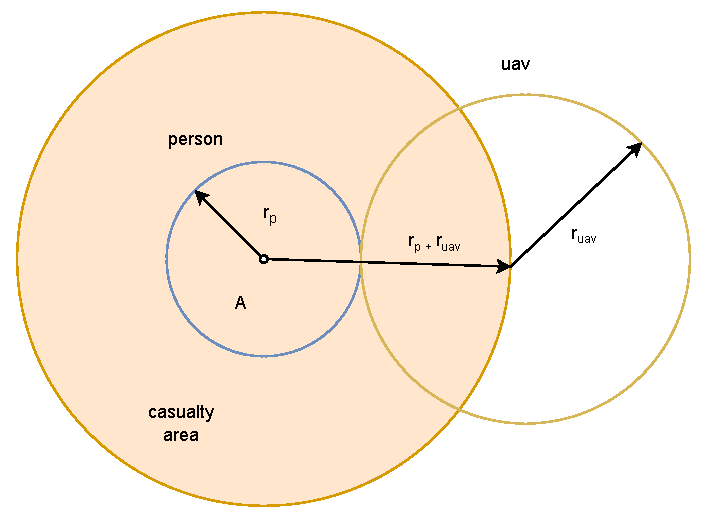
\includegraphics[width=0.75\textwidth]{General Image/OSM Drone-Area Exposed.pdf}
                \caption{Area exposed of casualty area}
            \end{figure}

            \begin{equation}
                A_{exp}(\theta) = \pi (r_p + r_{uav})^2 \sin (\theta) + (r_p + r_{uav})(h_p + r_{uav}) \cos (\theta)
            \end{equation}

            Where \(A_{exp}\) is an area exposed in \(m^2 \), $r_p$ and \(h_p\) is the average radius (0.3 \(m\)) and
            average height (182.5 \(m\)) of a person respectively in meter, $r_{uav}$ is the radius of the UAV in meter,
            and $\theta$ is the impact angle on the ground. This conservative computation takes into account the maximum
            radius of the UAV, ensuring a thorough evaluation of the impact area.

        \subsection{Recovery model}
            A recovery risk model for UAV is a model used to assess the likelihood of successful recovery of a UAV to a
            optimal or degraded operational state following a failure or malfunction. The model takes into account a
            variety of factors, the nature and severity of the failure, and the environment in which the recovery is
            taking place. The recovery risk model also takes into account the UAV design, capabilities and limitations.
            For example some UAV has parachute failsafe built into it. This parachute is then deployed when the control
            logic of the UAV detected major system breakdown. Some high-end UAV will enter a automatic landing or
            controlled crash into terrain before it deploys its parachute. Although not always it is a general rule of
            thumb that the UAV that has already equiped by parachute usually already has an advance flight controller.
            Please note that at the time of this writing, there are little to none database containing every specification
            of each highend drone.
                
            Although there is a significant in studying UAV recovery behaviour, only three researches that managed to
            include recovery model in its ground risk model. \cite{shelley_model_2016} calculated the safest highest
            possible flight altitude of the UAV based on its weight, or to be precised its resulted kinetic impact. It
            is showed that under any circumstances UAV with the weight over 1.5 kg must not be flown over a dense
            population. The study also give a benefit to equiping UAV with parachute will enable most UAV from only
            permitted to flown in tens of feet to 400 ft \ac{AGL}.

            The reasoning behind the small numbers of parachute descent being incorporate into GRM is because it assumes
            if the UAV already deployed its parachute, there are little to no threat to population. Hence, most of the
            reasearcher just give if else statements, where to just ignore its calculation if parachute is installed
            into the UAV. However some researcher goes into detail to see the effect of UAV impacting the surrounding
            area even with parachute, after all parachute can be drag by wind and still conatains an energy.

            \cite{primatesta_ground_2020} use parachute descent calculation based on the study from
            \cite{bleier_risk_2015}, where it calculate possible area where the UAV will land. \cite{bleier_risk_2015}
            use its calculation based on the relation ship of \(s = V \cdot t\), where \(s\) is distance, \(V\) is
            velocity and \(t\) is time. The relationship is expanded into include wind effect. Which resulted into
            equation \ref{eq:vsink} and \ref{eq:bleir}.

            \begin{equation}\label{eq:vsink}
                t_d = \frac{h} {V_{sink}}
            \end{equation}

            \begin{equation}\label{eq:bleir}
                \begin{pmatrix}
                    x \\
                    y
                \end{pmatrix}
                =
                \left( V_{\text{wind}} \pm \Delta V_{\text{wind}} \right) \frac{h}{V_{\text{sink}}}
                \cdot
                \begin{pmatrix}
                    \cos \left( \alpha_{\text{wind}} \pm \Delta \alpha_{\text{wind}} \right) \\
                    \sin \left( \alpha_{\text{wind}} \pm \Delta \alpha_{\text{wind}} \right)
                \end{pmatrix}
            \end{equation}

            Where \(t_d\) is time from deployed state to the ground, \(v_{sink}\) is the descent velocity,
            \(V_{wind}\) and \(\Delta V_{wind}\) is wind speed and random change in wind speed respectively,
            \(\alpha_{wind}\) and \(\Delta \alpha_{wind}\) is wind angle and random change in wind angle respectively

            We can see how the equation works from figure \ref{fig:area_parachute} below. Please not that
            \cite{bleier_risk_2015} only shows the equation for north down east coordinate system, where we use general
            cartesian coordinate for the figure. Back to the figure, if we view how the UAV is fell from the sky from a
            top down perspective, where the \(0,0\) is the point of deployment and has a wind affecting its descent
            trajectory. The UAV will take its time to be dragged into the ground by the wind to the red area, where the
            left most side is the furthest possible point, and vice versa for the right most side of the red area. 

            \begin{figure}[H]
                \centering
                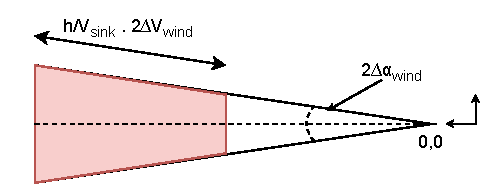
\includegraphics[width=0.75\textwidth]{General Image/OSM Drone-Landing zone.pdf}
                \caption{Range covered by parachute landing}
                \label{fig:area_parachute}
            \end{figure}

        \subsection{Stress model}
                The stress model explains the unpredictability of harmful circumstances occurring at a specific time and
            place. Or in other term what kind of harm are recieved by the population. For instance, stresses may be
            described as kinetic energy if the outcome to be calculated was human physical harm modeled in \ac{KE}.
            While secondary effects such as explosions and the release of hazardous chemicals will have distinct related
            stress qualities that need to be modeled differently. There are model proposed by \cite{ball_crash_2012} to
            analyze the consequences of heat radiation and explosions which often produces by chemical reaction. 18 of
            22 of the papers are using only kinetic energy as an only harm type in their ground risk model. This is not
            surprising since majority of the damage done into human body is kinetic energy based on the bomb explosion
            effect into human body reserach by \cite{harwick_approved_2007}.

            Depending on the kind of UAV, different stress factors that relate to one or more harmful processes may
            exist. Additionally, the UAV's characteristics and its trajectory may be changed to alter the stress profile
            at the site of impact. Through one or more harm mechanisms, the various stresses may be linked to the
            undesirable consequence. Examples of physical injury to humans include blunt force, penetration, crushing,
            blast, burns, lacerations.

            It should be mentioned that trauma generated by a blunt force collision is the main cause of injury taken
            into account by current models. It is possible that blunt force trauma is not the main cause of injury for
            UAV with tiny mass. Smaller multirotor UAV, for instance, have a higher tendency to lacerate individuals and
            inflict physical harm. In the stress model, laceration injuries must be taken into account, according to the
            \cite{small_aviation_2009}.

            The KE at impact was calculated by the models using a variety of mass and speed values, which is why the
            results of the stress models can differ from one another. For instance, \cite{ancel_real-time_2017} and
            other models simply assume the maximum velocity for estimating the impact energy for small UAV flying at low
            altitudes. Although using terminal velocity would be an overly conservative estimate, \cite{dalamagkidis_evaluating_2008} evaluation of the
            impact KE employs a similar assumption.

        \subsection{Exposure model}
            An exposure model is a method for determining how affected individual or property may be to dangers related
            to the use of UAV.

            A uniform exposure model is the model of population exposure that is most frequently utilized. The use of
            this approach overlooks possible population clustering within a specified geographic region and, as a
            result, averages the potential exposure factors contribution to the overall risk assessment. Such
            methodologies tend to overestimate or underestimate the risk value associated with the current setup because
            they do not provide sufficient information about the spatial and temporal distribution of the population.

            Models such as those created by \cite{burke_system-level_2011} and \cite{melnyk_third-party_2014} aim to add temporal features, acknowledging how individuals
            spend their days, taking such factors into consideration. An illustration of a thorough exposure model that
            emphasizes the time dependencies in population exposure is given by \cite{melnyk_third-party_2014}. Research conducted by \cite{klepeis_national_2001} found
            that individuals spent 68.7\% of their time at home, 7.6\% outside, 5.5\% in cars, 5.4\% at factories or
            offices, and another 12.8\% in various indoor settings. This data is used by \cite{melnyk_third-party_2014} to specify their exposure
            model along with the information.

            As expected population density data gathered for exposure model came from census, geographical data from
            satellite imagery. Depending on when each study was done and what regions were being analyzed, a different
            census data source was used. For instance, \cite{burke_system-level_2011} used data from the U.S. Census Bureau, and \cite{clothier_casualty_2007} used data
            from the Australian Bureau of Statistics. And to provide non uniform population data, cellular networks were
            used by \cite{ancel_real-time_2017} to create a near-real-time model of the population distribution.

        \subsection{Incident stress model}
            The incident stress model describes how much harm an individual is exposed to. Where in other term, how
            protected an individual from getting hit by the debris. Some papers such as \cite{primatesta_ground_2020},
            \cite{cour-harbo_ground_2020}, and \cite{dalamagkidis_evaluating_2008} to name a few, take into account an
            attenuating factor based on the sheltering effect to calculate how much kinetic energy a certain building
            can hold. In the model described by \cite{ball_crash_2012}, the amount of KE that is absorbed by the shelter
            as a result of its deformation, breaking, and movement is then subtracted from the overall risk posed by the
            system.

            Most of the shelter model in the paper who use it is split into four or five different type of building.
            From no shelter, sparse tree, small building, medium size building, and large building. Where small building
            typically describe a residential house or a small shop. Medium sized building where it describe a 2 stories
            building. And large building is from 3 stories and up. Based on investigations undertaken by the Columbia
            Accident and Investigation Board and the Department of Defense, \cite{melnyk_third-party_2014}, where it
            describe a method for calculating the risk from population distribution, most of the shelter are mostly
            residential structures and commercial buildings.

            As previously mentioned each of these shelter types has its attenuating factor, where it is just a
            coefficient factors to reduce the ammount of kinetic energy. It can be described as an simple proportional
            equation \ref{eq:shelter_factor} below

            \begin{equation}\label{eq:shelter_factor}
                S \cdot E_k
            \end{equation}

            Where \(S\) is a shelter factor ranging from 0 to 1.0, and \(E_k\) is kinetic energy in joule
            
        \subsection{Harm model}
            The harm model describe the severity of UAV impact towards the population. The harm model usually measured
            in probability of fatality given UAV impact to a person. The impact harm model can be categorized based on
            its severity from minor, major, and fatal injury.As previously mentioned many literature paper use kinetic
            impact energy as a variable when it comes to determining the fatality imposed by the UAV.  Of every injury
            mechanism, the most common studied harm mechanism is a blunt force trauma. According to
            \cite{shelley_model_2016}, the most likely impact injuries are injuries to the head, particularly skull
            fracture. 

            For various impact locations, the a charateristic of fatality probability model have been developed as as a
            function of kinetic energy by \cite{harwick_approved_2007}. The model describes the harm response of an
            average male, averaged over varying impact orientations, as a binomial regression function. Binomial
            distribution is a function that map a given input in this case kinentic energy to a false or true statement
            in this case a resulted fatality. Therefore, given a kinetic energy, does that energy can cause fatality to
            a person. 
            
            The binomial distribution is calculated using a sigmoid function, more commonly known as logistic curve.
            logistic curve probability of fatality described in \cite{shelley_model_2016} is presented in Eqn. 2.4.
            Where threshold is the impact energy associated with a 50\% probability of a fatality (measured in Joules),
            Energy imapct is the impact energy. A number of advancements over this standard equation have been presented
            by \cite{dalamagkidis_evaluating_2008} and \cite{shelley_model_2016} to name a few.

            \begin{equation}
                f(x) = \frac{1}{1+e^-\frac{(x-threshold)}{energy \ impact}}
            \end{equation}

            \begin{figure}[H]
                \centering
                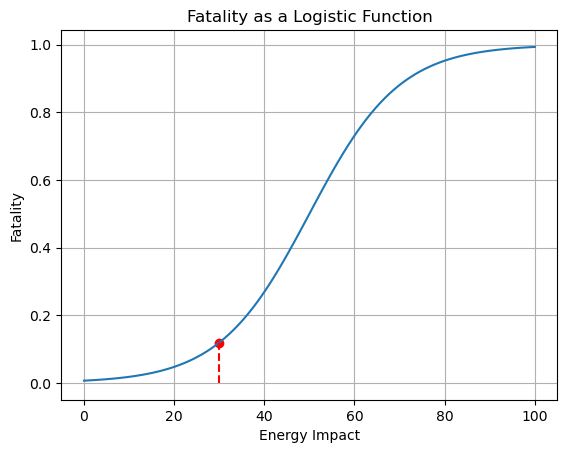
\includegraphics[width=\textwidth]{Plot/logistic_bounded.png}
                \caption{Generelized logistic fatality function given energy impact}
            \end{figure}


            \cite{magister_small_2010} makes use of a \ac{BC} that relates the kinetic energy on impact with the body's ability to
            tolerate the energy on impact, which is expressed using the \ac{AIS}.

        Overall, the use of ground risk models has the potential to significantly improve the safety and
        effectiveness of UAV operations. By identifying and prioritizing potential risks, ground risk models can help
        operators make informed decisions about how to mitigate or manage those risks. As the use of UAV continues to
        grow and expand into new applications, the importance of ground risk modeling is likely to increase as well.

        As an summary, think the ground risk model as a series of queestion asked in order. Where the questions are, how
        likely the will UAV fail, if the UAV fail where will it land, what does the descent landing looks like in
        ballistic, fly away, glide, or in parachute mode. If it land how likely is it to hit people in certain area. Are
        people in the somekind of shelter? if it does how safe is it if the drone hit them, does that hit cauase
        fatality?
        
    \section{Pathfinding Algorithms}

        This study not only for generating the ground risk map for the risk assesment but also measures and finds the
        path taken by the aircraft to find the least amount of risk and distance traveled required. That is why
        pathfinding algorithms are essential for UAV navigation, particularly for determining safe and efficient routes.
        There are multiple pathfinders, or in general, a method that is being used in the UAV industry as a navigation
        algorithm. All of these algorithms have different criteria, operating principles, and goals to complete.
        Therefore we are trying to reviews several common pathfinding algorithms, highlighting their advantages and
        limitations, and explains why the A* algorithm is selected for our study.
        
        Navigation algorithms are generally categorized into 2 parts based on the operational time: pre-operational
        algorithm and real-time operational algorithm. 

        \subsection{Bread-first search}
        \ac{BFS} is a fundamental algorithm that explores all nodes at the current depth level before moving on to the next
        level. This makes BFS an effective method for finding the shortest path in unweighted graphs. It works by
        starting at the root node and exploring all neighboring nodes. Then, it moves to the nearest nodes and explores
        their unexplored neighbors, continuing this process until the goal is reached.

        One of the main advantages of BFS is its guarantee to find the shortest path in terms of the number of edges in
        unweighted graphs. This algorithm is also straightforward and easy to implement. However, BFS can be very
        memory-intensive as it needs to store all nodes at the current depth level before proceeding to the next, which
        can be inefficient for large graphs or when memory resources are limited. Furthermore, BFS does not perform well
        on weighted graphs where the cost of traversing edges varies significantly \cite{cormen_introduction_2022}.

        \subsection{Depth-first search} 
        \ac{DFS} explores as far down a branch as possible before backtracking, making it useful for exhaustive searches
        of all possible paths. DFS starts at the root node and explores each branch to its fullest before moving to the
        next branch. This approach can be beneficial in situations where the complete path needs to be explored or
        specific deep paths are of interest.

        DFS is less memory-intensive than BFS since it only needs to store the nodes along a single path from the root.
        It is also simple to implement. However, DFS does not guarantee finding the shortest path. In cases of deep or
        potentially infinite graphs, DFS can get stuck in long paths, leading to inefficiency. This characteristic makes
        DFS less suitable for pathfinding where the shortest or optimal path is required \cite{knuth_art_1997}.

        \subsection{Djikstra's algorithm}
        Dijkstra's Algorithm is a widely used method for finding the shortest path in graphs with non-negative edge
        weights. It works by maintaining a set of nodes whose shortest distance from the source is known and repeatedly
        expanding the shortest known path by one edge. The algorithm uses a priority queue to efficiently select the
        node with the smallest tentative distance.

        Dijkstra’s Algorithm guarantees finding the shortest path in weighted graphs without negative weights, making it
        highly reliable for a variety of applications. It is efficient when implemented with a priority queue,
        especially for sparse graphs. However, the algorithm can be computationally intensive for very large graphs,
        which limits its scalability. For graphs with uniform weights, simpler algorithms like BFS may be more efficient
        \cite{dijkstra_note_2022}.

        \subsection{Greedy best-first search}
        Greedy Best-First Search is an algorithm that uses a heuristic to prioritize nodes that appear to be closest to
        the goal. Unlike Dijkstra’s Algorithm, which considers the cost to reach the current node and the estimated cost
        to reach the goal, Greedy Best-First Search only uses the heuristic estimate.

        The main advantage of Greedy Best-First Search is its speed, as it often finds a path faster than algorithms
        like Dijkstra’s. However, this speed comes at the cost of not guaranteeing the shortest path, especially in
        graphs where the heuristic is not perfectly accurate. This algorithm can be useful when a quick, approximate
        solution is needed rather than an exact shortest path \cite{russell_artificial_2016}.

        \subsection{Rapidly-exploring random tree}
        \ac{RRT} is a popular pathfinding algorithm used in robotics for motion planning in high-dimensional spaces. RRT
        works by randomly sampling points in the space and connecting them to the nearest node in the existing tree,
        effectively expanding the tree in unexplored regions.

        RRT is highly efficient in covering large search spaces and handling dynamic environments, making it suitable
        for real-time applications. It can be modified with various constraints, such as minimizing risk for UAV
        navigation. However, RRT does not always guarantee the shortest path and can produce suboptimal solutions that
        may require post-processing to refine \cite{lavalle_planning_2006}.





%---------------------------------------CHAPTER 3-------------------------------------
\chapter{Background Theory and Methodology}
    \section{General Overview}
        \begin{figure}[H]
            \centering
            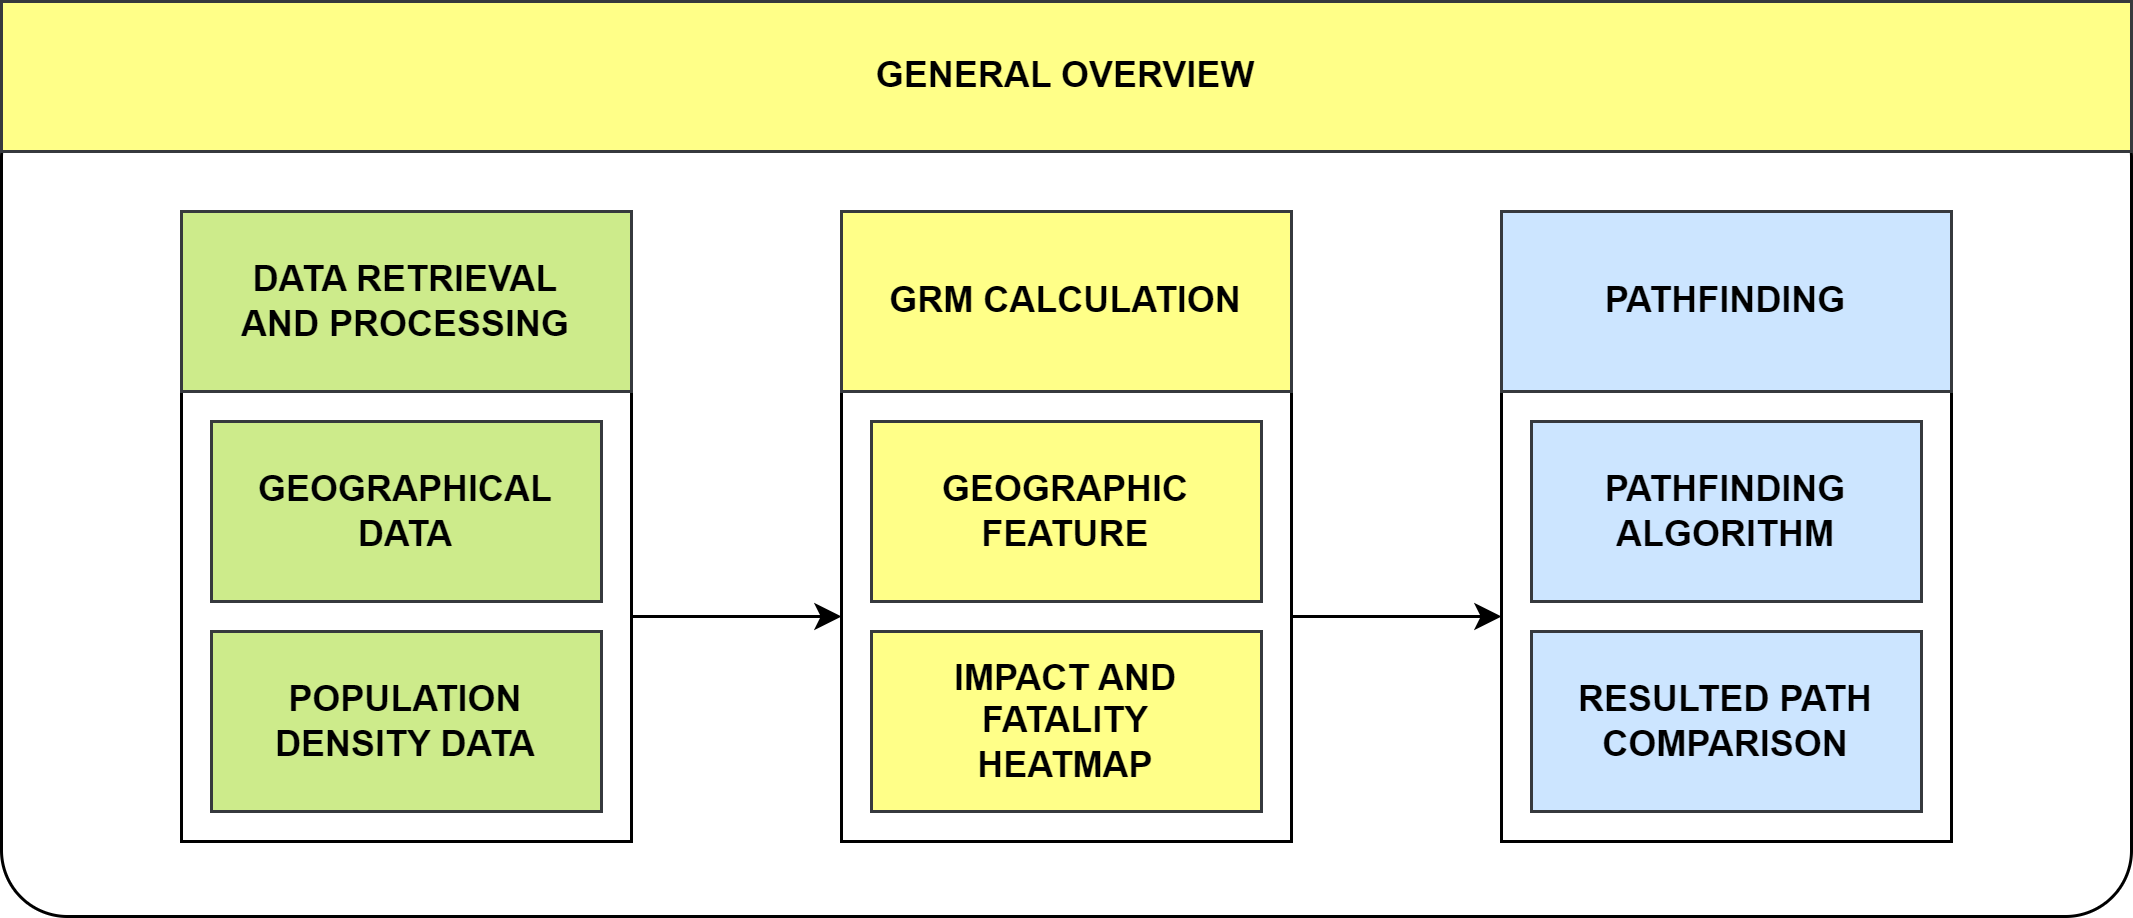
\includegraphics[width=\textwidth]{General Image/OSM Drone-General Overview.png}
            \caption{General overview}
        \end{figure}

        In general, there are three main objectives to create an optimal risk-aware flight path. These are data
        retrieval and processing, ground risk map calculation, and generating the most optimal path using the pathfinder
        algorithm.

        To collect necessary data, we are using free services provided by \ac{OSM} \cite{noauthor_openstreetmap_2022} to retrieve geographic
        data, and \ac{GHSL} \cite{noauthor_global_2023} to retrieve population density throughout the earth.

        The \ac{GRM} is calculated using geographic and population data, and also the type of aircraft that are being used in
        the calculation. The result would be descent location, impact energy, and fatality probability heat map. 
        
        After we compute and discretized the GRM. We find the optimal path with the least amount of risk using
        pathfinding algorithms, where the result would be compared.

    \section{Prerequisite data}
        \subsection{Online geographic data}
            OSM \cite{noauthor_openstreetmap_2022} is a collaborative project that aims to create a free, editable map of the world. It was founded in
            2004 and has since grown to become one of the largest and most popular sources of geospatial data.

            OSM is built on the idea that anyone can contribute to the map by adding and updating data. Users can add
            data using \ac{GPS} devices, aerial imagery, or by manually tracing over satellite imagery. The data is then
            stored in a database and made available under an open license, allowing anyone to use and share the data.

            There are multiple ways to use the OSM service. To retrieve the geographic data we can send the querry to
            Overpass \ac{API} and recieve the defaulted \ac{geoJSON} data. OSM also provide geocoding and reverse geocoding using
            Nominatim API.

        \subsection{Population data}
            GHSL \cite{noauthor_global_2023}. It is a dataset produced by the JRC (Joint Research Centre) of the European Commission that
            offers details on the distribution and location of human settlements worldwide.

            The GHSL classifies and examines patterns of urbanization and human settlement using new spatial data mining
            technologies and remote sensing data, such as satellite images. The dataset is periodically updated to
            reflect changes in urbanization and population growth and contains data on built-up areas, population
            density, and other indices of human presence.

            Overall, the GHSL is a valuable tool for comprehending the spatial dynamics and patterns of human settlement
            and can assist planners in making better-educated choices concerning urbanization and sustainable
            development.

        \subsection{Geographic Information System}
            Geographic and population data then stored and processed by \ac{GIS}, tools used
            for storing, manipulating, and visualizing geographic data. They allow users to analyze and understand spatial
            relationships, patterns, and trends in geographic data. 
            
            GIS consists of several key components:
            \begin{myitemize}
                \item Data: GIS uses data that is linked to a geographic location. This data can be in the form of
                points, lines, or polygons (areas) and can include attributes such as population, land use, or
                elevation.
                \item Hardware and software: GIS requires specialized hardware and software to store and analyze the
                data. This includes computers, servers, and specialized software such as ArcGIS or QGIS.
                \item Maps: GIS allows users to create interactive maps that can be used to visualize and analyze the
                data. Maps can be customized with different layers of information, such as roads, land use, and
                population density.
                \item Analysis: GIS allows users to perform spatial analysis on the data, such as calculating the
                distance between two locations or identifying patterns in the data.
            \end{myitemize}

            There are multiple GIS software suites, from standalone programs such as ArcGIS, and QGIS, to package base
            library for python, such as GeoPandas, Rasterio. In this paper we are going to use GeoPandas and Rasterio
            and its supporting libaries.

    \section{Risk map}
        The Risk map is a graphic representation depicting a potential risk associated with the UAV operation. Risk maps
        are divided equally in distance into cells. Each cell represented a bounded geographical location. The map can
        be represented by a \(M \times N\) size matrix, which each \(M \times N\) is the number of cells in each row and
        column respectively. Each \(\mathbf{R}(i,j)\) cell has centroid coordinates which represented the geographic
        location of \((x, y)\) in any coordinate reference system \ac{CRS}.

        If we use a slight notation abuse, which is \(\mathbf{R}(i,j)\), each cell coordinate \((i, j)\) is represented
        as a geographical location in which case shifted by \(x\) and \(y\) amount. Figure [Dex] illustrates the Risk map
        matrix.

        \subsection{Georeference layers}
            In a sense risk map is constructed by stacking layer of features, each layer itself is obtain by analyzing
            each geographical feature and population density to calculate the ground risk map. In this paper, multilayer
            frameworks are used based on the work of \cite{primatesta_ground_2020}. As the name implied, this framework contains multiple
            georeference layers. These layers are :
                \begin{myitemize}
                    \item \textbf{Population density layer}: Describes population density in the area.
                    \item \textbf{Obstacle layer}: Describes geographic features that can block aircraft flight paths
                    such as building height, or any other obstacle.
                    \item \textbf{Sheltering factor layer}: Describes geographic features that provide shelter for
                    humans in the area.
                    \item \textbf{No-Fly zone layer}: Describes geographic features in which aircraft cannot enter, such
                    as military base, or airport
                \end{myitemize}

        \subsection{Population density layer}
            The population density layer describes the population density and distribution in the area. It is one of the
            most crucial factors in the risk assessment is population density since it indicates how many individuals
            can be affected by a vehicle crash and how they are dispersed over the map.

            To conduct an accurate risk assessment it is necessary to provide population density data with fine
            resolution. since the likelihood of colliding with a person on the ground is particularly impacted by
            population density.

            The population data are frequently gathered by the government human settlement institute. However, this
            approach is not easily ported from country to country since different institutes produce population data
            differently. As previously mentioned above GHSL would be used in this paper, since it already has the global
            database.

            In this study, the population density layer is represented by a 2D georeference map with each cell
            corresponding to the value of population per cell area size with cell area in unit \(m^2\), therefore
            \(people/m^2\). Logically, the map would be in matrix form, \textbf{D}, with each cell element of
            \(\mathbf{D}(x, y)\).

            \begin{figure}[H]
                \centering
                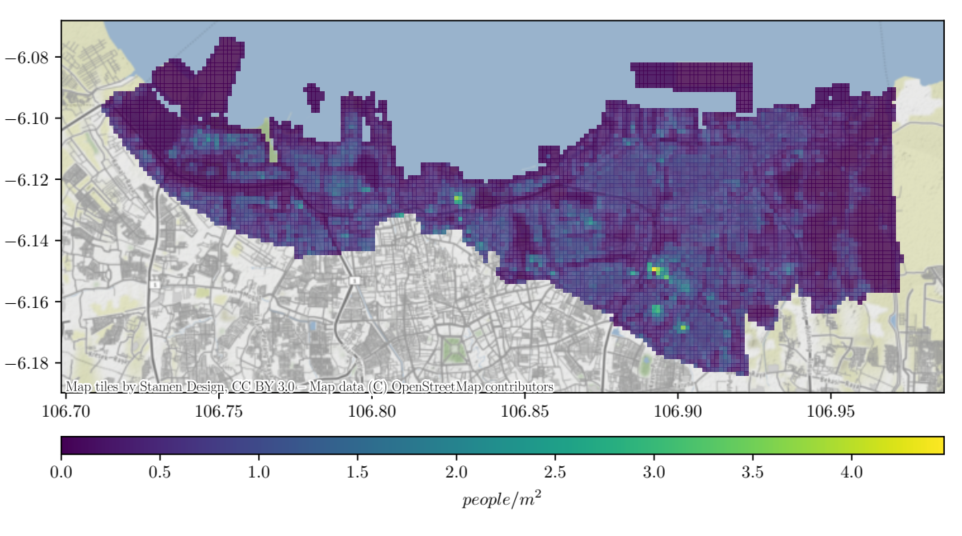
\includegraphics[width=\textwidth]{Plot/pop_dense.PNG}
                \caption{Population density map}
            \end{figure}

        \subsection{Obstacle layer}
            Obstacle layer describe which cell has contains a building or geographic feature which higher than flight
            altitude of UAV. the data can easily be gathered by filtering, and mark it as impasable terrain. since it is
            just another georeference layer, we can represent the as a matrix \(\mathbf{O}(x, y)\) which describe maximum height of
            building in a given cells.

            Noted that this layer does not explicitly accounted into risk factor analysis, but instead only for
            determining each cell is impasable for path finder.
            \begin{figure}[H]
                \centering
                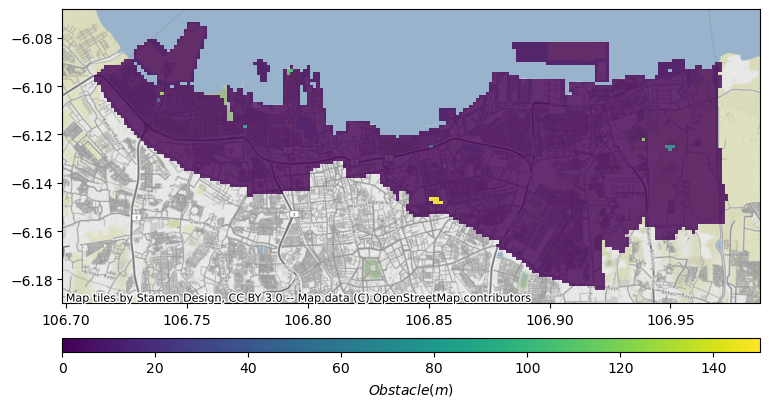
\includegraphics[width=\textwidth]{Plot/obstacle.png}
                \caption{Height obstacle map}
            \end{figure}

        \subsection{Sheltering factor layer}
            Sheltering Factor layer is a term for describing, the layer that focuses on assessing the presence and
            characteristics of physical structures or objects that can provide shelter. It is represented with a matrix
            \textbf{S}, where each element \(\mathbf{S}(x, y)\) assumes the sheltering factor value of the corresponding
            location.

            The sheltering factor layer takes into account factors such as the size, shape, material, and location of
            the structures or objects in the drone's operating environment. It aims to assess how these factors can
            influence the risk of fatality in case of failure.

            Unfortunately, it is impractical to evaluate the sheltering element in full detail in a study of this kind
            because it is a very complex scenario. The dynamic of drone collision is a complication in itself,
            particularly since detailed physical building features, like material or wall thickness, are recorded
            differently around the world.

            It is worsened by the fact that there are multiple studies with conflicting results when calculating the
            absorption of shelter since there is no consensus when defining the sheltering factor. Some studies by \cite{dalamagkidis_evaluating_2008}
            and \cite{primatesta_ground_2020} use a scale factor from 0 to 1, or 1 to 10 respectively, representing the energy absorption factor
            of a given building. While \cite{melnyk_third-party_2014} uses a study conducted by the \ac{DoD} \cite{harwick_approved_2007} regarding
            explosive study to measure the energy absorption capability.

            Even though it is tempting to use the method given by \cite{melnyk_third-party_2014} and DoD since it has the most accurate data. The
            study conducted by them is more suitable for singular operation-specific evaluation i.e. best case use for
            generating event tree, and not suited for generating risk map. There are also multiple problems when using
            this method, such as the lack of accurate data on building material geographic maps, especially when OSM do
            not provide a building material data, which would result in inaccurate measurement.

            From the previous statement, in this paper, we would use the scale factor proposed by \cite{klepeis_national_2001} and \cite{primatesta_ground_2020} as a
            foundation for sheltering factor risk generation. Since it provides a general method to calculate a risk
            factor. Table 3.1 is the shelter factor for types of features.
            
            \begin{figure}[H]
                \centering
                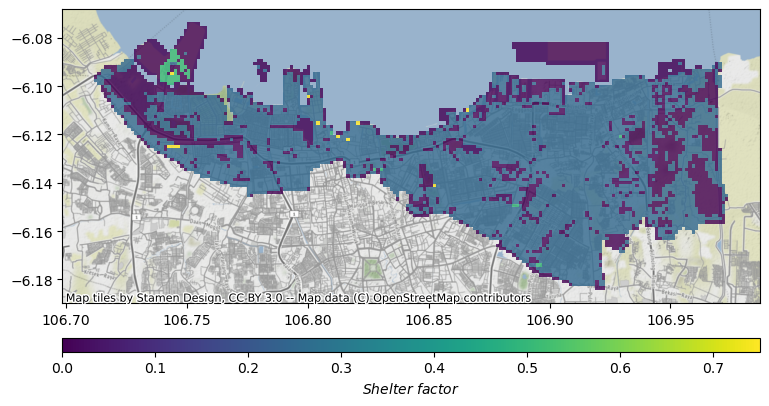
\includegraphics[width=\textwidth]{Plot/shelter_factor.png}
                \caption{Shelter factor map}
            \end{figure}


            \begin{table}[H]
                \centering
                \begin{tabular}{|p{4cm}|p{4cm}|}
                    Sheltering Factor & Type \\
                    \hline
                    0 & No shelters \\
                    \hline
                    0.25 & Sparse trees \\
                    \hline
                    0.5 & Low building \\
                    \hline
                    0.75 & High building \\
                    \hline
                    1.0 & Industrial building \\
                    \hline
                \end{tabular}
                \caption{Sheltering factor}
            \end{table}


        \subsection{No-fly zone layer}
            The No-fly zone layer refers to a component of a ground risk map or airspace map that delineates areas where
            drone flights are prohibited. The restrictions in these zones can include areas such as:
            \begin{myitemize}
                \item Regulation agency-defined areas, i.e.\ac{FAA}, and \ac{ICAO}. They restrict airports and military areas.
                \item Nature-sensitive areas, such as National Park where flying is restricted.
                \item Safety and security areas, very crowded public areas, such as the city center, or events.
                \item Operator-defined areas, where areas are restricted by the operator itself for various reason. 
            \end{myitemize}

            In this paper, the no-fly zone layer is a georeferenced map similar to the obstacle layer. And generally
            work in the same method to obstacle layers. The No-fly zone layers explicitly prohibit the flight of UAV by
            using two different values, -1 if flying is forbidden, and 0 if flying is allowed. The no-fly zone layer is
            represented by matrix \(\mathbf{F}(x, y)\) defined as:
            \begin{equation}
                \mathbf{F}(x, y) = 
                \begin{cases}    
                    -1 & \text{if flight is prohibited.} \\
                    0 & \text{if flight is allowed}
                \end{cases}
            \end{equation}

    \section{Ground Risk Assessment}
        In this research, the risk is described as the potential to cause harm of UAV to the population on the ground.
        quantified as the number of fatalities per hour of flight. The risk model is built upon a series of
        consecutively occurring events, each with its probability. These events are denoted as \(P_{event}\),
        \(P_{impact}\), and \(P_{fatality}\).

        \begin{equation}
            P_{casualty}(x) = P_{event}(x) \cdot P_{impact}(x) \cdot P_{fatality}(x)
        \end{equation}

        \(P_{event}\) represents the probability of the UAV losing control and descending into the ground. This paper
        considers four types of events: Ballistic, Unpowered Glide, Flyaway, and Parachute. Mathematical models are
        utilized to determine the probable impact area for each type of descent. It is important to note that these
        events are calculated independently of each other. Once the probabilities for each event are computed, they are
        summed up for each cell, resulting in the probability of the drone impacting that particular cell. This
        probability is described using a 2D \ac{PDF}. For further information on the descent
        models, please refer to Sections:\ref{sec:descent_events}. The two-dimensional PDF is utilized to calculate the
        probabilities of \(P_{impact}\) and \(P_{fatality}\), considering factors such as population density, sheltering
        factor layer, and impact velocities.

        After calculating the UAV crash location following an uncontrolled descent, we need to calculate the Pimpact
        which indicates the likelihood of the UAV strikes individuals. Where the population density and the impact
        exposure area can have its influence. And finally \(P_{fatality}\), which denotes the probability of fatal
        injuries occurring after a person has been impacted. It depends on the kinetic energy at the time of impact and
        the sheltering factor.

        The overall probability of casualty, \(P_{casualty}(x)\), is then computed. The \textbf{R} is a matrix
        containing calculated of said \(P_{casualty}(x)\) in every element of \(\mathbf{R}(x, y)\). This approach allows
        for the assessment of risk associated with UAS flights by considering various factors and probabilistic models
        for different events during the flight.

        \begin{figure}[H]
            \centering
            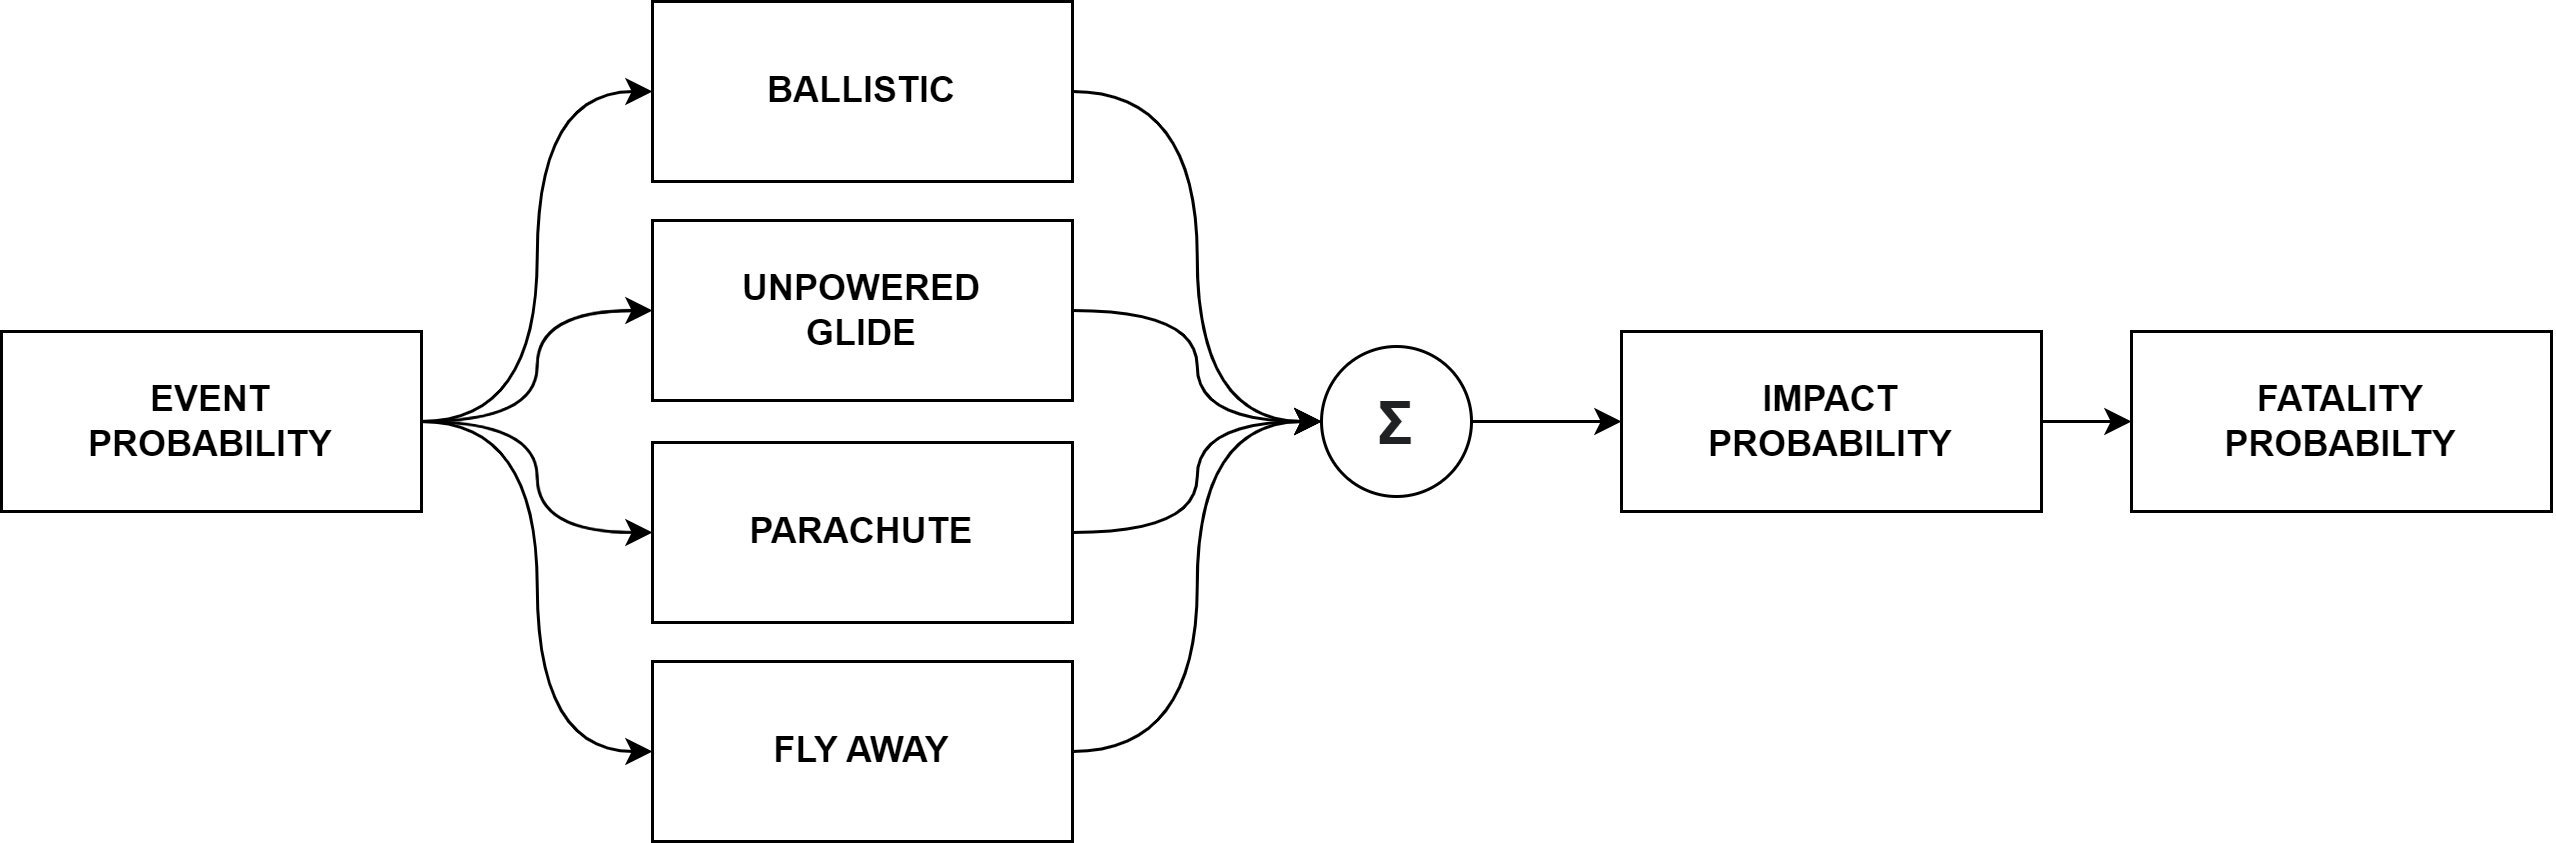
\includegraphics[width=\textwidth]{General Image/OSM Drone-LOGIC_SUM.png}
            \caption{General risk assesment flowchart}
        \end{figure}

        \subsection{Failure rate}
        The failure rate is a metric used to measure the reliability or average failure rate of a system or component.
        In this study, the MTBF would represent the failure rate. Where MTBF stands for Mean Time Between Failures. MTBF
        represents the average amount of time that elapses between consecutive failures of a system or component.
            
        MTBF is often expressed in time units, but usually it measures in hours, however, it can also be measured in
        other such as days or years. A higher MTBF value indicates a longer expected time between failures, suggesting a
        more reliable system or component.
            
        MTBF is typically calculated using historical failure data. Where this study using the assumption from, Shelley
        \cite{shelley_model_2016} and UAS Task Force \cite{noauthor_unmanned_2015} is set into 100 hours. 

        \subsection{Descent Event}\label{sec:descent_events} Information on how the UAV descended into the ground is
        required for ground risk management. The impact area and the kinetic energy at impact are determined according
        to the type of descent, which affects how the UAS falls to the ground. 
            
        The shape of a UAV has a great influence on how it falls, with fixed wings, generally glides down. While the
        multirotor fell following the ballistic trajectory. Both of which will influence the falling probability heat
        map. 
            
        These models below are employed to calculate a two-dimensional PDF that quantifies the likelihood of the UAS
        impacting the ground. The PDF takes into account uncertainties in the initial velocities (horizontal and
        vertical), drag coefficients, flight altitude, and flight direction. 
            
        Furthermore, the model generates a two-dimensional matrix containing the estimated horizontal and vertical
        impact velocities. These velocities are instrumental in computing the probabilities of impact (\(P_{impact}\))
        and fatality (\(P_{fatality}\)).

        \subsection{Ballistic Descent}
        The occurrence of ballistic descent arises when the aircraft experiences a catastrophic failure, such as a
        structural failure that results in the loss of most of its lift. Consequently, the vehicle undergoes a descent
        solely driven by the forces of gravity and drag.
        \begin{equation}
             m\dot{v} = m \mathbf{g} - c \cdot A \lvert \mathbf{v} \rvert \mathbf{v}
        \end{equation}
        
        The ballistic descent model used in this work is based on the standard second-order drag model. The model takes
        into account factors such as the mass of the UAV (\(m\)), a drag constant (\(c\)), area(\(A\)), air
        density(\(\rho\)), gravitational acceleration (\(g\)), and the vehicle's velocity vector (\(v\)). A study done by
        \cite{cour-harbo_ground_2020} provides greater details of the model that also considers uncertainties and variations in wind conditions.

        \begin{figure}[H]
            \centering
            \begin{subfigure}[b]{0.45\textwidth}
                \centering
                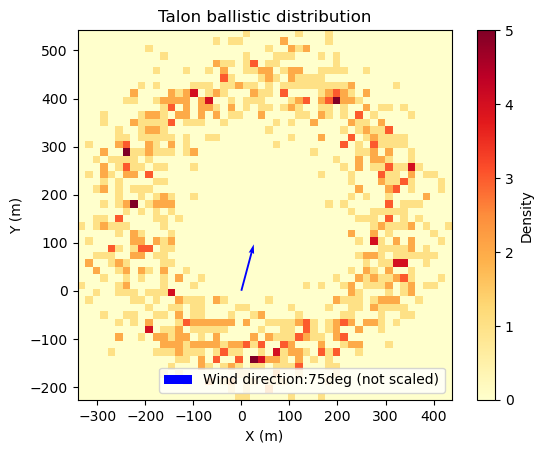
\includegraphics[width=\textwidth]{Plot/talon/ballistic.png}
                \caption{Fixed wing ballistic descent}
                \label{fig:fixed_wing}
            \end{subfigure}
            \hfill
            \begin{subfigure}[b]{0.45\textwidth}
                \centering
                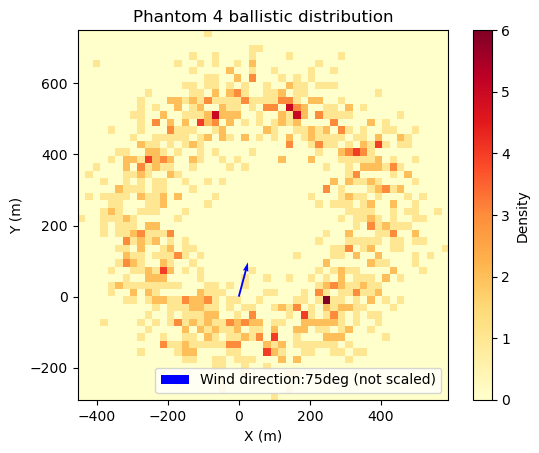
\includegraphics[width=\textwidth]{Plot/phantom4/ballistic.png}
                \caption{Multirotor ballistic descent}
                \label{fig:multirotor}
            \end{subfigure}
            \caption{Ballistic descent by aircraft type}
            \label{fig:ballistic_descent}
        \end{figure}

        \subsection{Glide Descent}
        Uncontrolled glide may arise depending on the configuration of the aircraft. It is an event when UAV flight
        profiles are governed solely by the glide ratio or autorotation angle. This event could happen when aircraft
        loses its power but still retains most of its lift capability.
            
        In the case of a fixed-wing aircraft, this event arises from a loss of thrust or power affecting the flight
        control surfaces. For a single rotorcraft, it occurs when there is a loss of thrust on the main rotor, causing
        the aircraft to descend using autopiloted autorotation. However, multi-rotor cannot enter unpowered glide,
        instead, it enters ballistic descent.
            
        During the uncontrolled glide event, the horizontal distance traveled is computed using the simple formula
        \(dist(h) = \gamma{h}\) , where h represents the flight altitude and \(\gamma\) represents the glide ratio

        \begin{figure}[H]
            \centering
            \begin{subfigure}[b]{0.45\textwidth}
                \centering
                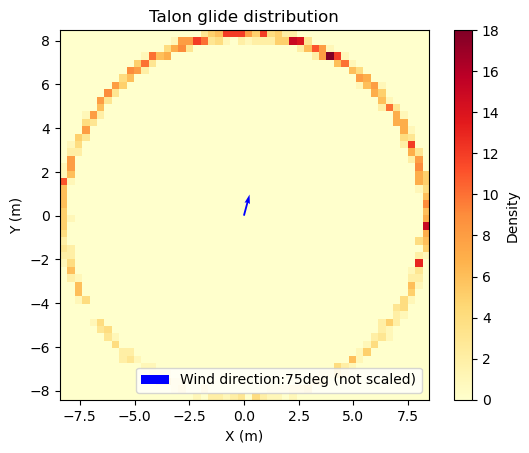
\includegraphics[width=\textwidth]{Plot/talon/glide.png}
                \caption{Fixed wing glide descent}
                \label{fig:fixed_wing}
            \end{subfigure}
            \hfill
            \begin{subfigure}[b]{0.45\textwidth}
                \centering
                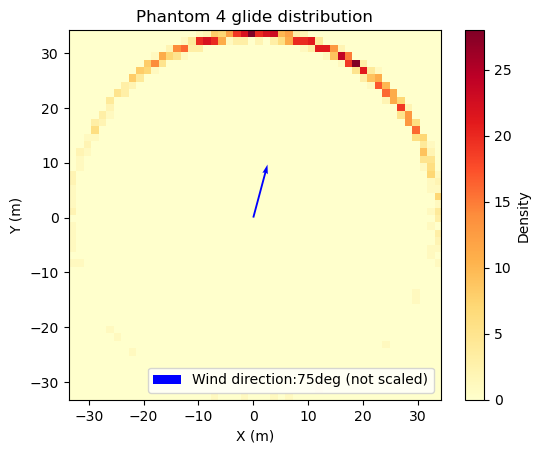
\includegraphics[width=\textwidth]{Plot/phantom4/glide.png}
                \caption{Multirotor glide descent}
                \label{fig:multirotor}
            \end{subfigure}
            \caption{Glide descent by aircraft type}
            \label{fig:ballistic_descent}
        \end{figure}

        \subsection{Fly away}
        The fly-away event occurs when the operator loses complete control over the UAV, while the onboard flight
        control maintains the stability of the vehicle. As a result, the UAS can fly in any direction until it crashes
        on the ground. This event is modeled based on a reference paper \cite{la_cour-harbo_quantifying_2019} , which proposes a model comprising two
        components. Firstly, the probability of ground impact decreases linearly with the distance from the UAS position
        until reaching the maximum distance the vehicle can travel. Secondly, the vertical motion of the vehicle is
        taken into account, with a higher probability of ground impact near the UAS position, modeled as a normal
        distribution centered around the UAS position. These two contributions are combined linearly using a scaling
        factor.
            
        In this study, equal probabilities are assumed for both scenarios to be conservative. It is assumed that the
        fly-away event terminates with an uncontrolled glide descent. Unlike other descent events, the fly-away event
        can involve motion in all directions. Figure 16 presents the results of the fly-away event.

        \begin{figure}[H]
            \centering
            \begin{subfigure}[b]{0.45\textwidth}
                \centering
                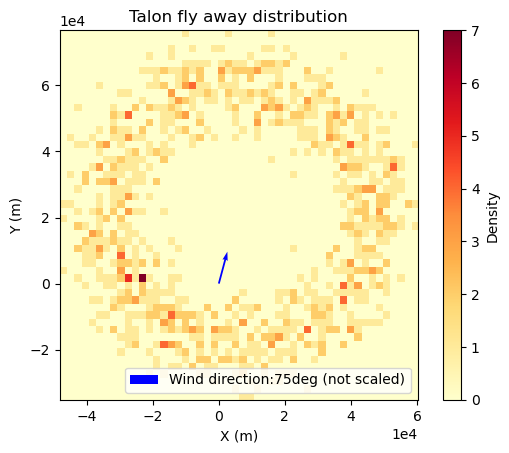
\includegraphics[width=\textwidth]{Plot/talon/fly_away.png}
                \caption{Fixed wing fly away descent}
                \label{fig:fixed_wing}
            \end{subfigure}
            \hfill
            \begin{subfigure}[b]{0.45\textwidth}
                \centering
                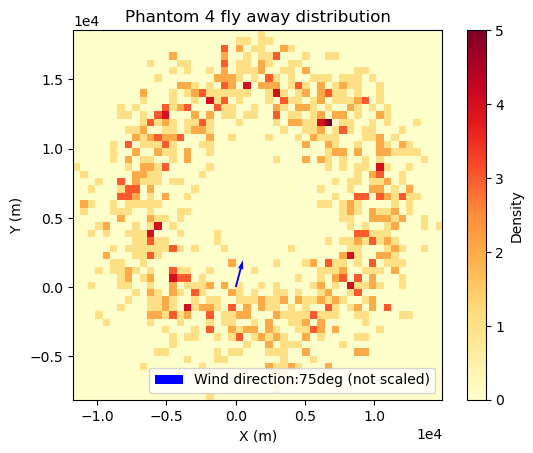
\includegraphics[width=\textwidth]{Plot/phantom4/fly_away.png}
                \caption{Multirotor fly away descent}
                \label{fig:multirotor}
            \end{subfigure}
            \caption{Fly away descent by aircraft type}
            \label{fig:ballistic_descent}
        \end{figure}

        \subsection{Parachute}
        The parachute descent starts when the UAV flies downward while the parachute is fully extended. The power plants
        are typically shut off and the parachute is opened when a problem occurs. After the emergency detection and the
        parachute fully opening, there is, however, a small delay. The only factors affecting the drop at this point are
        the parachute's aerodynamic features, which are intended to slow the vertical speed.
            
        To model this event, a methodology described in a referenced paper \cite{la_cour-harbo_quantifying_2019}is employed. The authors of the paper
        consider factors such as the mass of the vehicle, as well as the physical properties of the parachute, including
        its area and drag coefficient. Notably, the presence of wind significantly alters the descent dynamics,
        affecting the direction and velocity of the descent.

        \begin{figure}[H]
            \centering
            \begin{subfigure}[b]{0.45\textwidth}
                \centering
                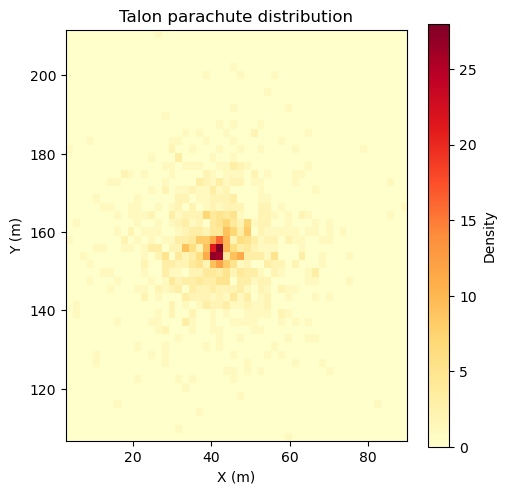
\includegraphics[width=\textwidth]{Plot/talon/parachute.png}
                \caption{Fixed wing parachute descent}
                \label{fig:fixed_wing}
            \end{subfigure}
            \hfill
            \begin{subfigure}[b]{0.45\textwidth}
                \centering
                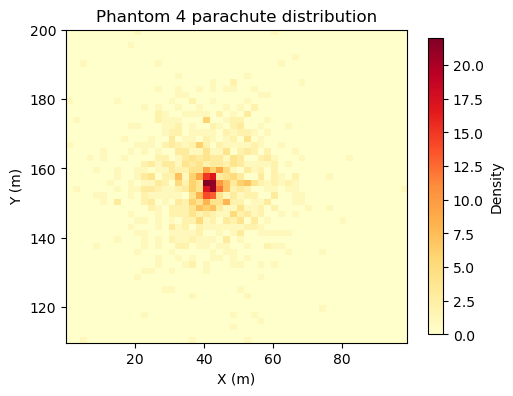
\includegraphics[width=\textwidth]{Plot/phantom4/parachute.png}
                \caption{Multirotor parachute descent}
                \label{fig:multirotor}
            \end{subfigure}
            \caption{Parachute descent by aircraft type}
            \label{fig:ballistic_descent}
        \end{figure}

        \subsection{Wind effect}
        The wind is one of the important variables in creating a ground risk map since wind speed and direction is
        determined the impact location of each descent event. Where the wind data can be received from weather forecast
        information before the operation.
            
        Noted that this study assumes and applies constant wind speed and direction when simulating the descent event.
        This assumption arose when the wind effect usually encompasses a large local area which is often greater than
        medium to micro-sized UAV. Added to that, the wind only affected only the descent event and not when the drone
        is normally operating.
            
        \subsection{Probability of Impacting an Individual}
        The \(P_{impact}\) is the probability of a UAV striking individual. This parameter is important because, when
        used in conjunction with the population density parameter previously discussed, it determines the number of
        people exposed to risk on the ground in the event of an impact.

        \begin{equation}
            P_{impact}(x,y)=\rho(x,y) \cdot A_{exp}
        \end{equation}

        The \(P_{impact}\) equation describe the population density \(\rho\) and exposure area Aexp
            
        Similar to sheltering factor, there is no standard approach when calculating the affected area. However, there
        are two distinct approaches that most researchers find useful, the empirical method and the geometric method.
            
        Empirical methods are the method that uses regression to calculate impact area based on the size or the weight
        of an aircraft. While the geometric method uses the general dimension of the aircraft to calculate the impact
        area.

        Research done by \cite{melnyk_third-party_2014} uses the regression method from \cite{ale_assessment_2000}, based on the accident data of large aircraft to
        calculate the impacted area. However, this regression is created using aircraft weight of more than 1500kg. This
        can result in underestimating the lethality of common UAV operations which weigh less than 500kg.
            
        A study done by \cite{aalmoes_conceptual_2015} proposes two types of solutions. empirical regressionand geometric approach. Which stated
        that, above 500kg the calculation should use the empirical method, or geometric approach if less than 500kg. The
        empirical data obtained by the Netherland Aerospace Laboratory, when researching the helicopter crashes
        behavior, resulted in \ref{eq:radial} relation. While the geometric approach \ref{eq:human_impact} is using
        human impact model.

        \begin{equation}\label{eq:human_impact}
            A_{exp}(m) = 230 \ln \left( \frac{m}{1000} \right) + 330
        \end{equation}

        \begin{equation}\label{eq:radial}
            A_{exp}(\theta) = 2 (r_p + r_{uav}) \frac{h_p}{\tan(\theta)} + \pi (r + r_p)^2
        \end{equation}

        Where \(A_{exp}\) is in \(m^2\), with m is kg, \(\theta\) is impact UAV impact angle. And \(r_{uav}\) is UAV
        radius , \(h_p\) is person height, and rp is person radius all in \(m\),

        \subsection{Probability of Fatality}
        The probability of fatality, denoted as \(P_{fatality}\), represents the likelihood that an impact on a person
        will result in a fatality. Calculating this probability is challenging due to the various complexities involved
        in an impact event. The human body reacts differently to different types of impacts, and UAV crashes can involve
        factors such as blunt impact, lacerations, or chemical explosions caused by the battery. As a result, variables
        like velocity and mass do not have a simple correlation to the severity of injuries, as the human body's
        response varies depending on the specific body part affected. This lack of consensus on the calculation method
        for fatality probability arises from the difficulty of accounting for all the intricacies and variations in
        impact events. However, it is generally accepted to correlate kinetic impact energy to measure the
        \(P_{fatality}\).

        \begin{equation}\label{eq:fatality}
            P_{fatality} = \frac{1}{1 + e^{-k(E_{imp} - E_{thres})}}
        \end{equation}

        \ref{eq:fatality} is a generalized equation based on the logistic function, where the function maps a value of
        impact energy Eimp to the probability of fatality, with Ethres is an energy value that has a probability to
        cause fatality above 50\%. On average, 58 joules of energy can cause a fatality based on the table below.

        \begin{table}[H]
            \centering
            \begin{tabular}{|p{6cm}|p{1.5cm}|p{1.5cm}|p{4cm}|}
                \hline
                Information & Value & Unit & Source \\
                \hline
                Energy for hazardous debris & 45 & Joule & \cite{cole_hazards_1997} \\
                \hline
                Energy required by fragment for 90\% probability of fatality & 120 & Joule & \cite{cole_hazards_1997} \\
                \hline
                Energy required by fragment to be hazardous to human & 58 & Joule & \cite{gonzales_faas_2017} \\
                \hline
            \end{tabular}
            \caption{Energy correlate to fatality}
        \end{table}

        This study would be using more comprehensive $P_{fatality}$ Equation \ref{eq:fatality}, with $\alpha$ as
        threshold energy to cause 50\% probability of fatality in a medium level of shelter $S \geq 0.6$, and $\beta$ is
        the threshold energy needed to cause fatality when in a non-sheltered area ($S \leq 0.1$).

        \begin{equation}\label{eq:fatality}
        P_{fatality}(x, y) = \frac{1}{1 + \sqrt{\frac{\alpha}{\beta} \left[ \frac{\beta}{E_{imp}(x,y)} \right]^{\frac{1}{4S(x,y)}}}}
        \end{equation}
        
        The kinetic energy is computed as:
        
        \begin{equation}\label{eq:kinetic_energy}
        E_{imp}(x, y) = \frac{1}{2} m \cdot v_{imp}(x, y)^2
        \end{equation}
        
        Equation \ref{eq:fatality} is based on Equation \ref{eq:fatality} from a study conducted by \cite{dalamagkidis_evaluating_2008} and \cite{primatesta_ground_2020}.
        Although it is not accounted for chemical and thermal factors as in \cite{melnyk_third-party_2014} and \cite{harwick_approved_2007}, we argue that since both \cite{melnyk_third-party_2014}
        and \cite{harwick_approved_2007} only suitable for evaluating per single event and not for generating ground risk map.

    \section{Finding optimal path}
        After creating a risk map, the next objective is to find the optimal flight path with the least amount of risk.
        From a naive method point of view, computing flight path is quite easy since 99\% of the operation is only a
        straight path from point A to point B since there is little to no obstacle. Instead, the risk factor has a
        bigger impact on the Pathfinder compared to real physical obstacles.

        There are many types of pathfinder algorithms with each of its advantage, disadvantage, and its most effective
        usage of operation. In this paper, we would be using A* and Dijkstra's algorithm to find the optimal path and
        compare each algorithm. There is an explanation in section [A] for reasons why we are not going to use other
        algorithms.

        \subsection{Problem statement}
        \textbf{Given:}
        \begin{myitemize}
            \item A grid with dimensions \(M \times N\), where each cell represents a location in the grid.
            \item A start cell \(S\) and a goal cell \(G\) in the grid. 
            \item Each cell in the grid has an associated risk factor (a non-negative real value) that represents the
            level of risk or danger associated with that cell.
        \end{myitemize}

        \textbf{Objective:} Find the shortest path from the start cell \(S\) to the goal cell \(G\) that minimizes the
        cumulative risk factor along the path.
        
        \textbf{Formally, let:}:
        \begin{myitemize}
            \item Let \(G = (V, E)\)  be the graph representation of the grid, where \(V\) represents the set of cells
            and \(E\) represents the set of edges connecting adjacent cells in the grid.
            \item Let \(w(u, v)\) be the weight or cost associated with an edge \((u, v)\) in E. In this case, the
            weight \(w(u, v)\)  represents the risk factor of moving from cell \(u\) to cell \(v\).
            \item Let \(d(u)\) represent the shortest path distance from the start cell \(S\) to cell \(u\).
        \end{myitemize}

        The problem is to find the shortest path \(P = (S, v1, v2, . . . , G)\) that minimizes the cumulative risk
        factor along the path, which can be represented by the sum of the weights along the path:

        \begin{equation}\label{eq:weighted_graph}
            min \sum w(v_i,v_{i+1})
        \end{equation}

        subject to:
        \begin{myitemize}
            \item \(P\) is a valid non negative weighthed path from \(S\) to \(G\) in the graph \(G\).
            \item \(d(G)\) is minimized.           
        \end{myitemize}
        The objective is to find the path \(P\) that minimizes the cumulative risk factor, taking into account the risk
        factors associated with each cell in the grid.
            
        This problem can be solved using various algorithms such as Dijkstra's algorithm, A*, or even extensions like
        Risk-Aware A* that consider risk factors in the pathfinding process.
            
        Noted that the specific formulation and constraints of the problem may vary depending on additional
        considerations such as movement constraints, specific risk factor calculations, and other domain-specific
        requirements. The above problem statement provides a general framework for finding the shortest path based on
        risk factor in a grid system.

        \textbf{Graph}
        Before using any pathfinder algorithm, the grid map must be defined in the graph. In computer science and
        mathematics, a graph is a data structure that represents a collection of interconnected nodes, called vertices,
        \((V)\), and the relationships between them, called edges, \((E)\).
            
        A graph consists of two main components: Vertices (Nodes): These are the fundamental units of a graph and
        represent entities or objects. Each vertex is typically labeled with a unique identifier or value. Edges: These
        represent the connections or relationships between vertices. An edge connects two vertices and can be either
        directed or undirected.
            
        A directed edge has an orientation or a specific direction, while an undirected edge does not. Edges can also
        have weights or costs associated with them to represent the strength of the relationship or distance between
        vertices.
            
        A grid typically falls into the category of a regular graph or a lattice graph. A regular graph is a graph in
        which every vertex has the same number of neighbors. In a grid, each cell is typically connected to its adjacent
        cells, resulting in a regular graph structure. The number of neighbors depends on the dimensionality of the
        grid.
            
        The grid system, with its regular arrangement of cells and connectivity between adjacent cells, can also be
        considered a form of lattice graph. A lattice graph is a specific type of regular graph that forms a
        lattice-like structure. A lattice graph consists of a regular arrangement of vertices in a grid-like pattern,
        where each vertex is connected to its adjacent vertices.

        \subsection{Dijkstra's algorithm}
        Dijkstra's algorithm is a well-known and widely used algorithm for finding the shortest path between a given
        source node and all other nodes in a graph. It guarantees optimality, meaning it always finds the shortest path,
        as long as the graph has non-negative edge weights.

        Dijkstra's algorithm uses a cost function to calculate the shortest path from a given start node to all other
        nodes in a graph. The distance in Djikstra's case is represented as a cost function of \(g(x)\).

        \begin{equation}
            g(x)=min(g(x_{goal}),g(x_n))
        \end{equation}

        The function \(g(xn)\) represents the shortest distance from the start node to a given node \(x_n\) in the
        graph. It is initialized to a very large value, often infinity, for all nodes except the start node, which is
        assigned a distance of 0.
        
        \begin{equation}\label{eq:costfunction}
            g(x_n)=\sum_{i=1}^{n-1}g(x_{i-1})+c(x_{n-1},x_n)
        \end{equation}

        where, $\sum_{i=1}^{n-1} g(x_{i-1})$ is all combined cost from a start node to the current node, and $c(x_{n-1},
        x_n)$ is a risk-weighted cost function, which describes to

        \begin{equation}
        c(x_{n-1}, x_n) = \frac{r(x_{n-1}) + r(x_n)}{2} \cdot d(x_{n-1}, x_n)
        \end{equation}
        
        where the risk $r_x$ is the average between two nodes, and $d(x_{n-1}, x_n)$ is an euclidean distance between
        two nodes.
        
        The algorithm iteratively selects the node with the minimum distance among the unvisited nodes and updates the
        distances of its neighboring nodes if a shorter path is found. This process continues until all nodes have been
        visited or until the goal node is reached, depending on the specific problem requirements.

        By continuously updating the distances of nodes based on the weights of the edges, Dijkstra's algorithm ensures
        that it explores paths with lower total costs, gradually converging towards the shortest path from the start
        node to each node in the graph.

        \begin{algorithm}
        \caption{Dijkstra’s Algorithm}
        \begin{algorithmic}[1]
        \Function{Dijkstra}{start, goal}
            \State distances $\gets$ \{\}
            \State previous $\gets$ \{\}
            \ForAll{node in graph}
                \State distances[node] $\gets \infty$
                \State previous[node] $\gets$ undefined
            \EndFor
            \State distances[start] $\gets 0$
            \State queue $\gets$ PriorityQueue()
            \State queue.insert(start, 0)
            \While{queue is not empty}
                \State current $\gets$ queue.pop\_min()
                \If{current is goal}
                    \State \Return ReconstructPath(previous, current)
                \EndIf
                \ForAll{neighbor of current}
                    \State distance $\gets$ distances[current] + cost(current, neighbor)
                    \If{distance $<$ distances[neighbor]}
                        \State distances[neighbor] $\gets$ distance
                        \State previous[neighbor] $\gets$ current
                        \State queue.insert(neighbor, distance)
                    \EndIf
                \EndFor
            \EndWhile
            \State \Return Failure
        \EndFunction
        \Statex
        \Function{ReconstructPath}{previous, current}
            \State path $\gets$ [current]
            \While{previous[current] is defined}
                \State current $\gets$ previous[current]
                \State path.prepend(current)
            \EndWhile
            \State \Return path
        \EndFunction
        \end{algorithmic}
        \end{algorithm}

        \subsection{A* algorithm}
        A* algorithm is an extension of the Dijkstra algorithm and uses a heuristic function to guide the search. From
        \ref{eq:heuristic} we can see that the addition of heuristic function \(h(x_n)\). Noted that the implementation
        of \(g(x)\) is similar to previously mentioned in \ref{eq:costfunction}.

        The cost function can be represented as:
        \begin{equation}\label{eq:heuristic}
            f(x)=g(x_n)+h(x_n)
        \end{equation}

        where:
        \begin{myitemize}
            \item \(f(n)\) is the total estimated cost of node n,
            \item \(g(n)\) is the actual cost from the start node to node n,
            \item \(h(n)\) is the heuristic estimate of the remaining cost from node n to the goal node.
        \end{myitemize}

        The cost function in the A* algorithm typically consists of two components: the actual cost to reach a vertex
        from the start node, and the heuristic estimate of the remaining cost from the vertex to the goal node. The sum
        of these two components represents the total estimated cost from the start node to the goal node through a
        particular vertex.
            
        The heuristic estimate, \(h(x_n)\), must be an admissible (underestimating) heuristic function that provides an
        estimate of the remaining cost from node n to the goal node. Admissibility is a requirement for the algorithm to
        be able to look for the best solution in the graph. If admissibility is not implemented, overestimation might
        occur in the algorithm, and it may overlook nodes that would lead to the optimal solution.
            
        The solution for admissible heuristic implementation is based upon the paper from
        \cite{primatesta_risk-aware_2019}. Where the author \textit{dialed down} the heuristic value by multiplying it
        by the risk cost between \(x_{goal-1}\) and the \(x_{goal}\) itself, this is to ensure conservative heuristic
        admissibility.

        \begin{equation}
        \begin{aligned}
        h(x_n) = \frac{r(x_n) + r_{\text{min}}}{2} \cdot \text{dist}(x_n, x_{n+1}) + \text{dist}(x_{n+1}, x_{\text{goal}-1}) r_{\text{min}} \\
        + \frac{r(x_{\text{goal}}) + r_{\text{min}}}{2} \cdot \text{dist}(x_{\text{goal}-1}, x_{\text{goal}})
        \end{aligned}
        \end{equation}

        By summing the actual cost and the heuristic estimate, the A* algorithm prioritizes nodes with lower total
        costs, resulting in a search that tends to explore paths that are likely to be closer to the goal. This
        heuristic-guided exploration helps to efficiently find the shortest path from the start node to the goal node.

        To summarize, when there is a single unique optimal path, A* can discover it more efficiently than Dijkstra's
        algorithm by utilizing an admissible heuristic function. While Dijkstra's algorithm has the capability to
        eventually find the absolute optimal path given sufficient time. By comparing the results of A* and Dijkstra's
        algorithm, we can assess the performance of A*.

        \begin{algorithm}
        \caption{A* Algorithm}
        \begin{algorithmic}[1]
        \Function{AStar}{start, goal}
            \State openSet $\gets \{\text{start}\}$
            \State closedSet $\gets \{\}$
            \State cameFrom $\gets \{\}$
            \State gScore $\gets \{\}$
            \State hScore $\gets \{\}$
            \State fScore $\gets \{\}$
            \State gScore[start] $\gets 0$
            \State hScore[start] $\gets$ \Call{heuristic}{start, goal}
            \State fScore[start] $\gets$ gScore[start] + hScore[start]
            \While{openSet is not empty}
                \State current $\gets$ node in openSet with the lowest fScore
                \If{current is goal}
                    \State \Return \Call{ReconstructPath}{cameFrom, current}
                \EndIf
                \State openSet $\gets$ openSet \textbackslash\ $\{$current$\}$
                \State closedSet $\gets$ closedSet $\cup$ $\{$current$\}$
                \ForAll{neighbor in \Call{Neighbors}{current}}
                    \If{neighbor in closedSet}
                        \State \textbf{continue}
                    \EndIf
                    \State tentativeGScore $\gets$ gScore[current] + \Call{cost}{current, neighbor}
                    \If{neighbor not in openSet \textbf{or} tentativeGScore $<$ gScore[neighbor]}
                        \State cameFrom[neighbor] $\gets$ current
                        \State gScore[neighbor] $\gets$ tentativeGScore
                        \State hScore[neighbor] $\gets$ \Call{heuristic}{neighbor, goal}
                        \State fScore[neighbor] $\gets$ gScore[neighbor] + hScore[neighbor]
                        \If{neighbor not in openSet}
                            \State openSet $\gets$ openSet $\cup$ $\{$neighbor$\}$
                        \EndIf
                    \EndIf
                \EndFor
            \EndWhile
            \State \Return Failure
        \EndFunction
        \Statex
        \Function{ReconstructPath}{cameFrom, current}
            \State path $\gets$ [current]
            \While{current in cameFrom}
                \State current $\gets$ cameFrom[current]
                \State \Call{prepend}{current, path}
            \EndWhile
            \State \Return path
        \EndFunction
        \end{algorithmic}
        \end{algorithm}

    \section{UPX, UAV Pathfinding eXtension}

        \begin{figure}[H]
            \centering
            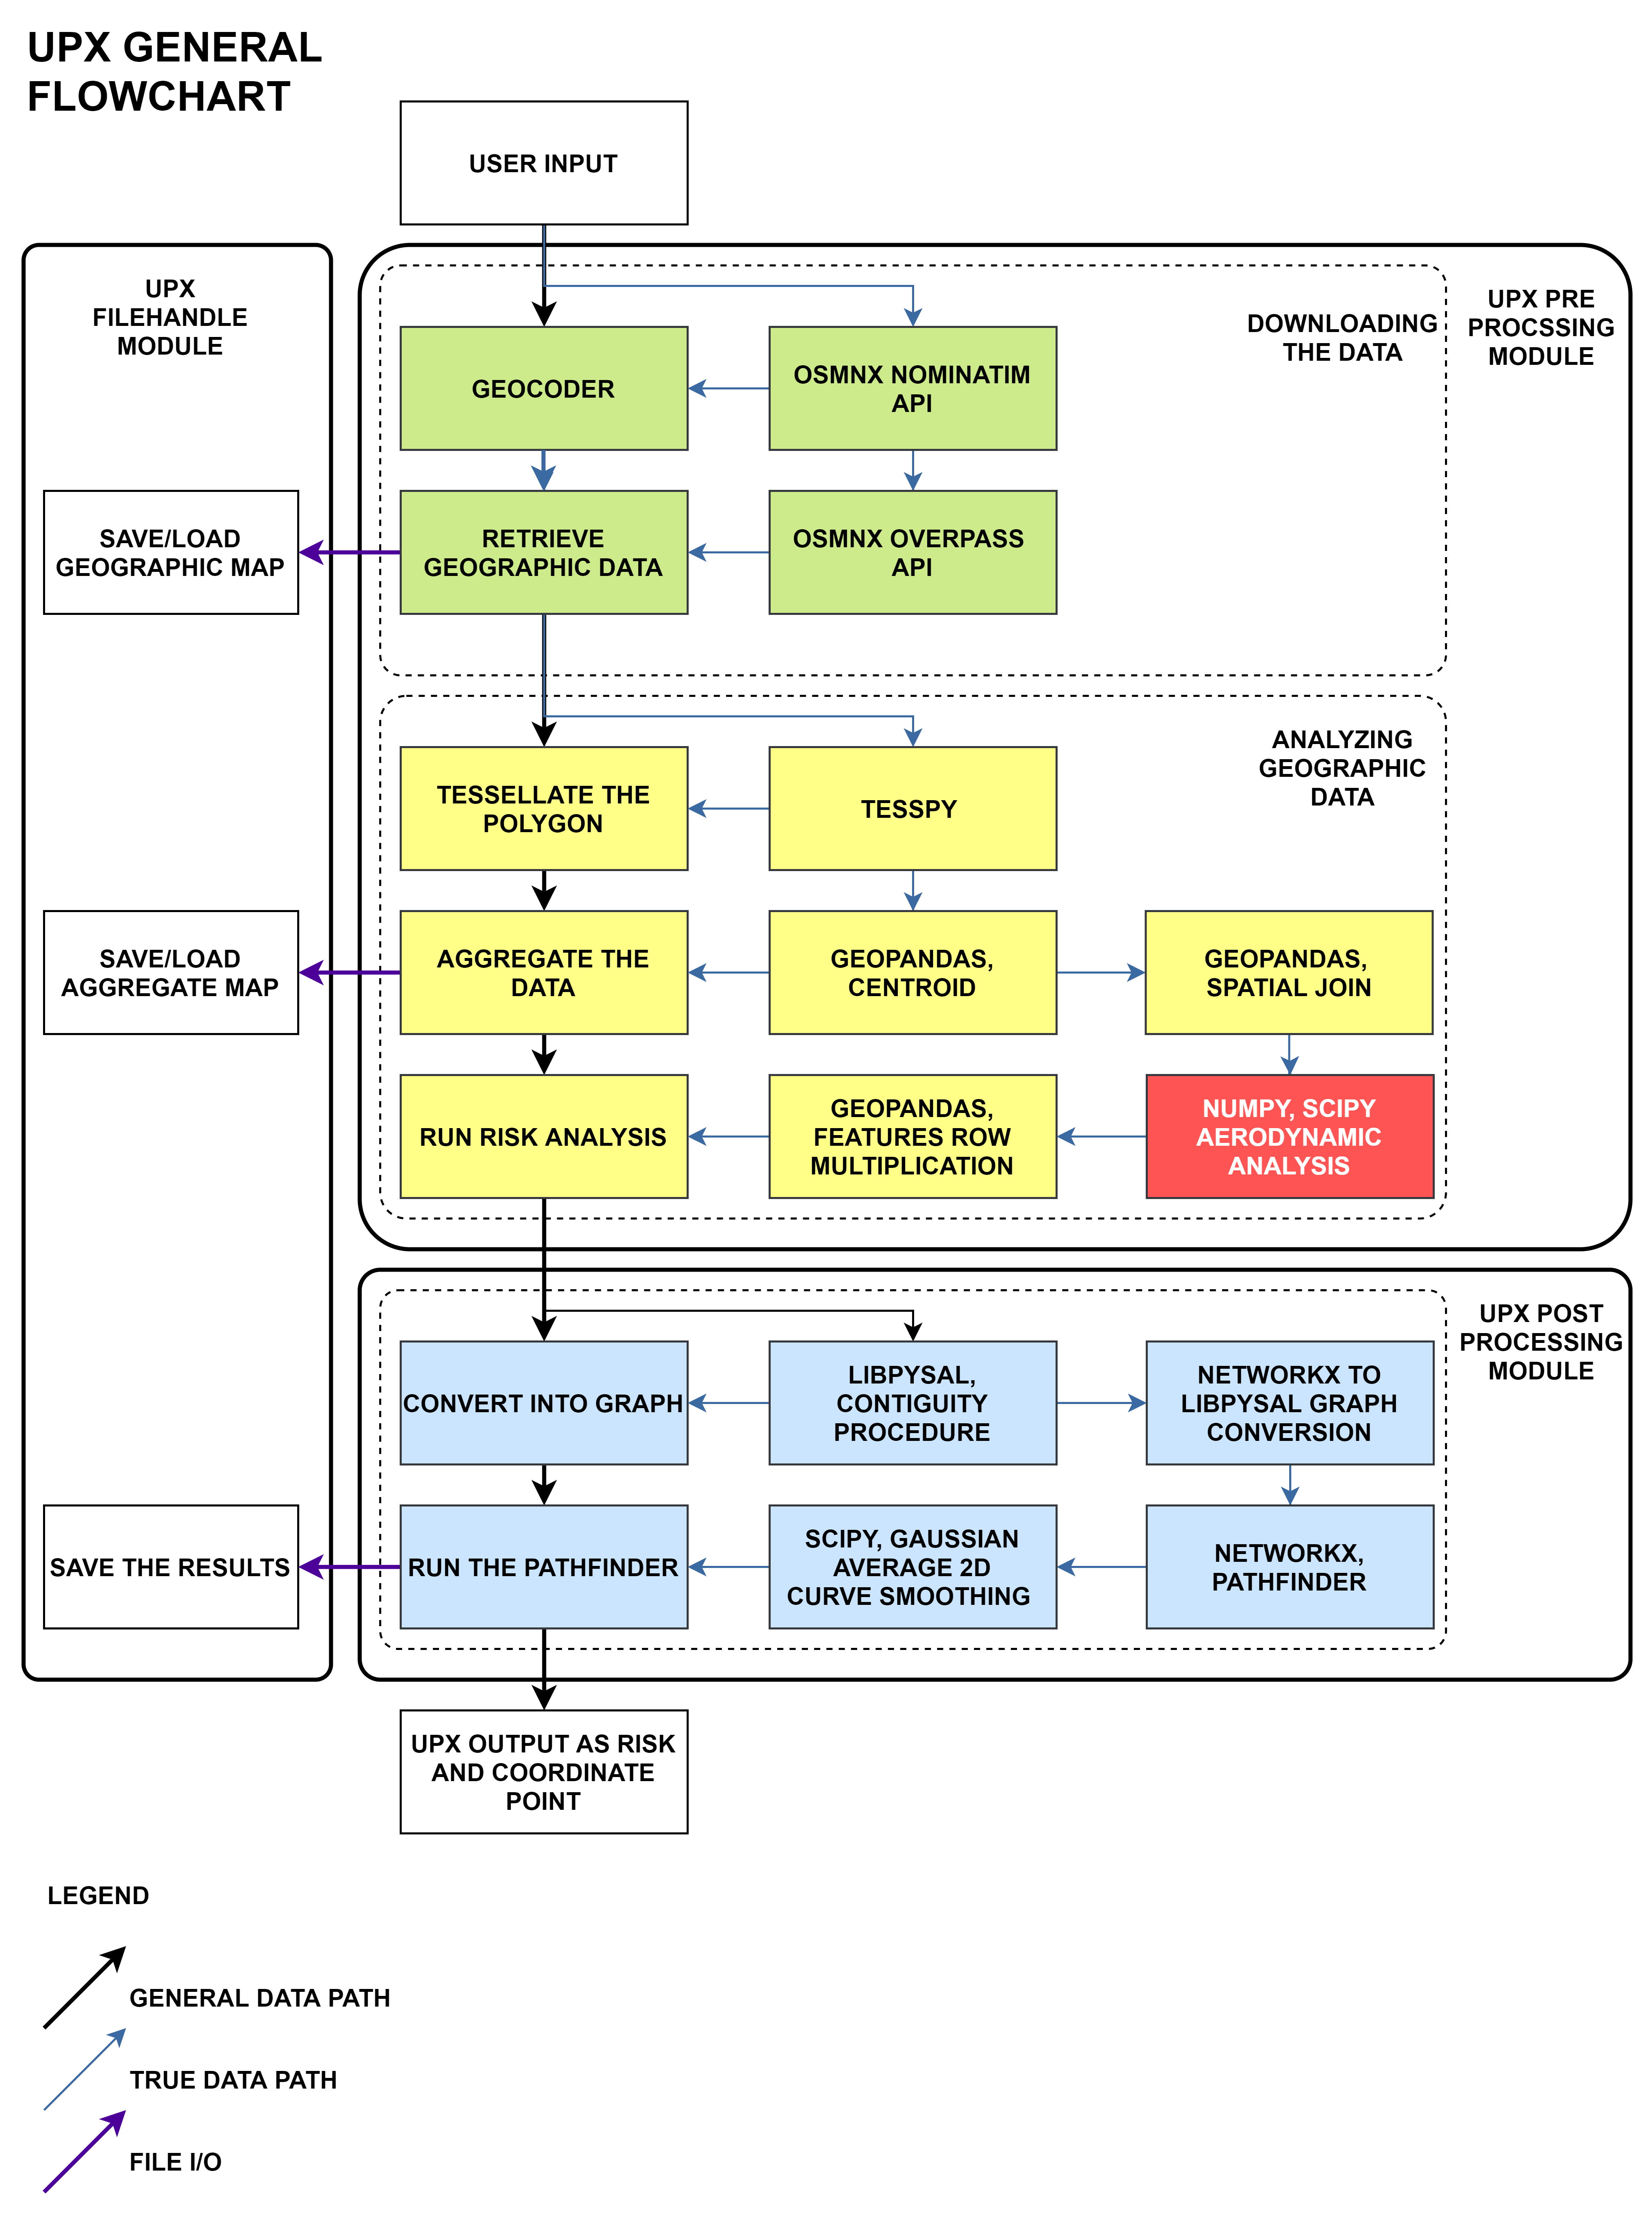
\includegraphics[width=\textwidth]{General Image/UPX GENERAL FLOWCHART.png}
            \caption{UPX architecture design}
            \label{fig:UPX_arch}
        \end{figure}
        
        UAV Pathfinding eXtension, UPX, is both a python libraries and application to find the optimal risk-informed
        flight path. In general, UPX works by retrieving geographic data from OSM, receiving geographic data, then being
        discretized and aggregated. The risk map is then converted into a graph for the pathfinding algorithm. The risk
        mentioned Risk in UPX is rules to determine the probability of fatality in case the UAV happens to malfunction
        and falls in that area.
            
        UPX was built based on the concern of negative consequences of increase frequency of UAV flying in urban areas.
        While UPX is intended to be used to aid UAV operation, its library can be used in any type of aircraft as long
        they provide aerodynamic parameters and aircraft performance data. However, some caveats would be explained in
        the UPX limitation below.

        \subsection{Limitation}
        Firstly, UPX is strictly for a preliminary assessment only. It does not handle real-world phenomena such as
        sudden wind gale, rain, storm, or other aircraft that, unfortunately, are present in the path of the UAV. For
        that reason only, we hope the pilot practice safe flying and the UAV itself is provided with the failsafe
        feature.

    \section{UPX Python and packages}
        \subsection{Python}
        Python is an interpreted programming language. Interpreted language has the benefit of being an easier language
        to compare to a compiled language. Added to this, it has massive scientific-related packages and libraries.
        Combine with quick deployment and its STEM library, it is a perfect choice for engineering, mathematics, and
        physics analysis. Based on previous criteria it is a great choice for creating UAV path planner applications and
        libraries.
            
        While Python indeed has a great advantage. Unfortunately, its comparatively easy language came with a great
        price. An interpreted language is inherently slow, 8 to 100 times slower compared to C/C++ language. Base Python
        language also cannot use more than one thread because its GIL, Global Interpreter Lock, prevents the threads
        from sharing memories and create a parallel workload. Fortunately, most of the heavy calculation is handled by
        the c/c++ library, where Python uses the caller function to launch the libraries.

        \subsection{GeoPandas}
        GeoPandas is one of the GIS libraries built for tabulating and analyzing geographicalspatial analysis in python.
        GeoPandas itself can be regarded as the extension of Pandas library, where Pandas is general tabular data
        processor. GeoPandas has geographic spatial and attribute related function such as overlay, spatial join,
        clipping to group, aggregate, and measure geospatial data.
            
        GeoPandas exports and imports files in standard GIS-supported files such as geoJSON, the file, and the Shapely
        object, to name a few. In Python GeoPandas tabular data is called GeoDataFrame, and GeoSeries. What
        differentiates between GeoDataFrame and regular DataFrame is the addition of a geometry column. The geometry
        column can contain Multi/Polygon, Multi/Linestring, and Point shapes.

        \subsection{Shapely}
        Shapely is a geomeytry calculation and manipulation packages available for python. Many of geospatial function
        in GeoPandas relies on Shapely itself. Overlay, clipping, spatial binary combination in GeoPandas can be found
        in Shapely. In this paper Shapely is being uses to create custom filter for heat map function of aircraft
        falling probability.

        \subsection{Tesspy}
        Tesspy, a tesselation library for Python. Its purpose, as the name implies, is to create a tesselated polygon.
        Tesspy can be used as long as the polygon object is derived from the Shapely object. Tesspy offers type of
        tessellated map that commonly use for geospatial processing. Square grid, hexbin, Voronoi city block, and
        adaptive square is the type of tesselated maps, to name a few.

        \subsection{OSMnx}
        OSMNx is a combination of OSM and NetworkX. OSMNx is mainly being uses to create graph representation of the
        road network. It uses the GeoPandas data frame, to build the network, as long as the roads in question are
        connected at least with another road. But for this paper, OSMNx is only being used as a geocoder and reverse
        geocoder to retrieve GeoPandas data.

        \subsection{NetworkX}
        To create a graph structure, NetworkX provides the necessary function to do that. NetworkX offers graph
        creation, graph traversal algorithms, and graph manipulation. The graph, as previously mentioned, in a
        combination of nodes and edges. The A* pathfinder for the UAV Path finder also uses the NetworkX built-in A*.

%---------------------------------------CHAPTER 4-------------------------------------
\chapter{Results}
    \section{Ground risk map generation}
        \subsection{UAV Specification}
        In this study, we are going to analyze the risk factor of multirotor and fixed-wing UAV. In comparison, Talon
        and Parrot Disco are fixed-wing. While DJI Phantom 4 and DJI Inspire 2 are multirotor. Four of them are chosen
        since they are generally known as a go-to standard in the commercial drone industry. Each category is also
        differentiated into two different sizes, where Talon and Inspire 2 are the large size, while Phantom 4 and Disco
        are much smaller UAV. All properties are obtained from manufacturer design specifications.
            
        As for the aerodynamic properties of these drones, we are using a very simple drag model. This will not include
        an Induced drag since we cannot predict every possible angle of attack. It is also beneficial to use simplify
        drag model since it would give a higher impact velocity, which increases the impact energy and results in a much
        more conservative value.
            
        It is worth mentioning the mechanic of the glide model in this risk analyzer. Since only fixed wings are capable
        of gliding, and to an extent, a variable-pitch helicopter by autorotation, it is almost impossible to make a
        glide descent on a fixed-pitch propeller multirotor. Where for the multirotor, ballistic descent is the more
        likely outcome, even though there is little to no damage in the aircraft. It is then assumed that a glide
        descent, and to an extent a glide speed in multirotor, as a low powered horizontal descent where the power is
        barely sustaining a hover maneuver

        \begin{table}[H]
            \centering
            \begin{tabular}{| l | l | l | l | l |}
                \hline
                \textbf{Specification} & \textbf{Talon} & \textbf{Parrot Disco} & \textbf{Phantom 4} & \textbf{Inspire 2} \\
                \hline
                Type & Fixed wing & Fixed wing & Quadcopter & Quadcopter \\
                Mass (kg) & 3.75 & 0.75 & 1.4 & 4.25 \\
                Front area (m$^2$) & 0.1 & 0.07 & 0.02 & 0.04 \\
                Radius (m) & 0.88 & 0.575 & 0.2 & 0.4 \\
                Maximum flight time & 1.25 h & 45 min & 20 min & 25 min \\
                Ballistic drag coefficient & N(0.9, 0.2) & N(0.9, 0.2) & N(0.7, 0.2) & N(0.7, 0.2) \\
                Horizontal initial speed (m/s) & N(18, 2.5) & N(15, 2.5) & U(0, 15) & U(0, 20) \\
                Vertical initial speed (m/s) & 0 & 0 & 0 & 0 \\
                Glide speed (m/s) & 16 & 12 & 7.5 & 10 \\
                Glide ratio & N(12, 2) & N(2.7, 0.8) & N(2.7, 0.8) & N(2.7, 0.8) \\
                Parachute drag coefficient & N(13, 0.2) & N(0.9, 0.2) & N(0.9, 0.2) & N(0.9, 0.2) \\
                Parachute area & 1 & 0.5 & 0.5 & 0.5 \\
                \hline
            \end{tabular}
            \caption{UAV Specifications}  % Add caption here
        \end{table}

    \section{Objective}
    The ground risk would be performed in North Jakarta, Indonesia. The place is chosen for its dense population, an
    assortment of building heights, large water bodies, and multiple residential and commercial zone areas. Shown in \ref{fig:map}
        
    And for the operation itself, the UAV would be flying from Pluit Village to Jakarta Sailing Vocational School. This
    objective is chosen based on the criteria previously mentioned.
        
    We would compare the performance of the Risk A* Algorithm vs the Normal A* algorithm. We do not include Djikstra's
    algorithm in this section since the A* algorithm provided by the NetworkX library is already admissible and able to
    obtain optimal pathways.
        
    It is worth mentioning the normal A* is the same for all types of aircraft since aircraft properties are only
    important in Risk A* in generating various descent PDFs.

    \begin{figure}[H]
        \centering
        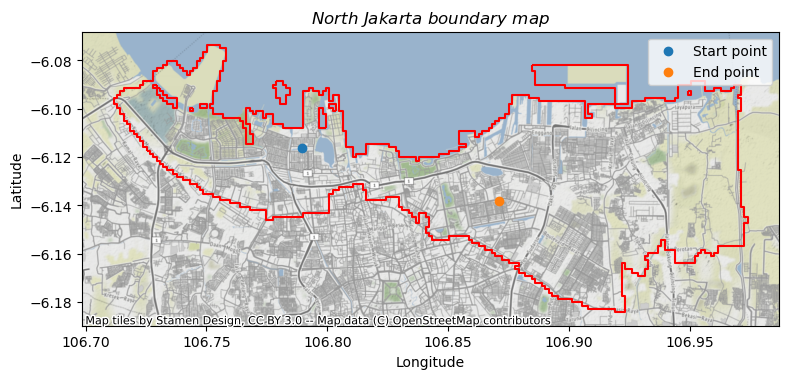
\includegraphics[width=\textwidth]{Plot/route.png}
        \caption{Operation objective}
        \label{fig:map}
    \end{figure}

    \section{PDF risk map}
        \subsection{Talon}
        \begin{figure}[H]
            \centering
            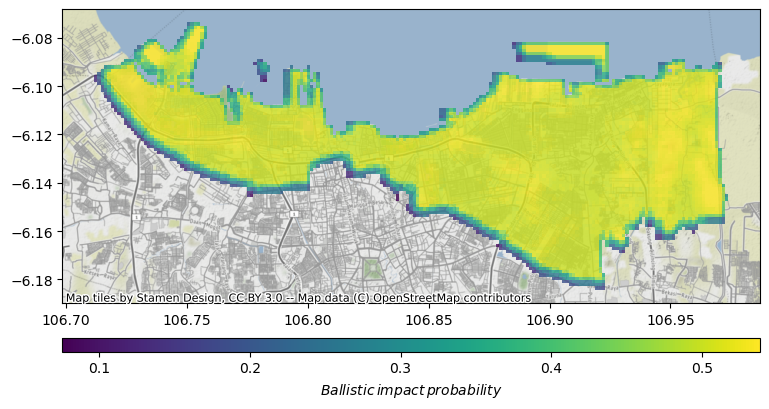
\includegraphics[width=\textwidth]{Plot/talon/ballistic_fpdf.png}
            \caption{Talon ballistic PDF}
        \end{figure}
        \begin{figure}[H]
            \centering
            \includegraphics[width=\textwidth]{Plot/talon/glide_pdf.png}
            \caption{Talon glide PDF}
        \end{figure}
        \begin{figure}[H]
            \centering
            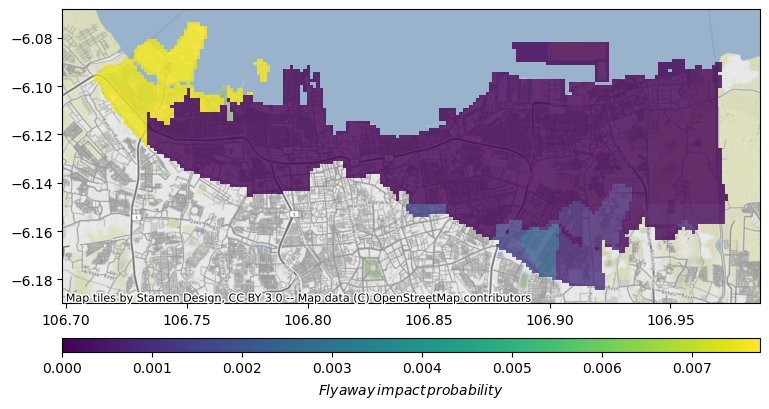
\includegraphics[width=\textwidth]{Plot/talon/fly_away_pdf.png}
            \caption{Talon fly away PDF}
        \end{figure}
        \begin{figure}[H]
            \centering
            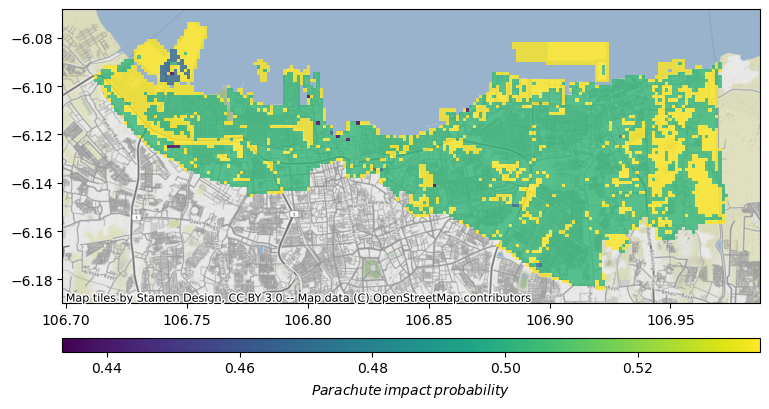
\includegraphics[width=\textwidth]{Plot/talon/parachute_pdf.png}
            \caption{Talon parachute PDF}
        \end{figure}
        \begin{figure}[H]
            \centering
            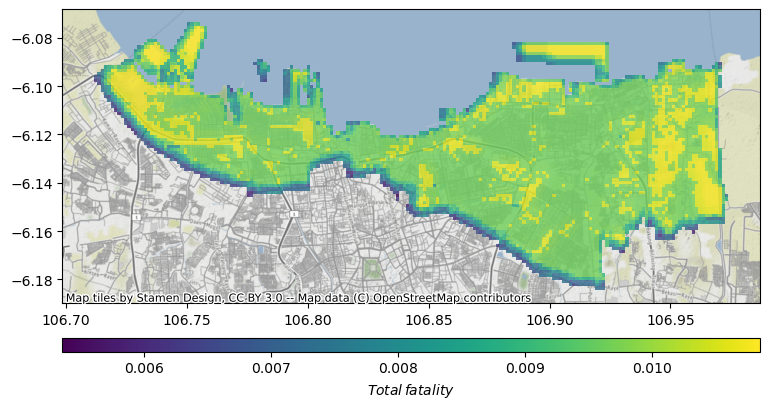
\includegraphics[width=\textwidth]{Plot/talon/total_fatality.png}
            \caption{Talon fatality risk PDF}
        \end{figure}

        \subsection{Parrot Disco}
        \begin{figure}[H]
            \centering
            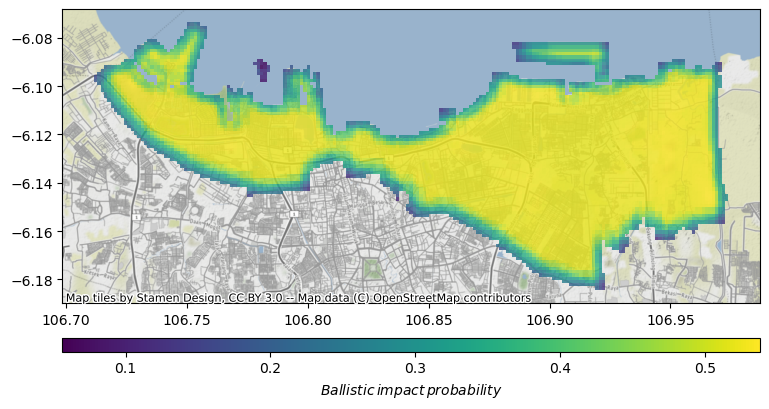
\includegraphics[width=\textwidth]{Plot/parrot/ballistic_pdf.png}
            \caption{Disco ballistic PDF}
        \end{figure}
        \begin{figure}[H]
            \centering
            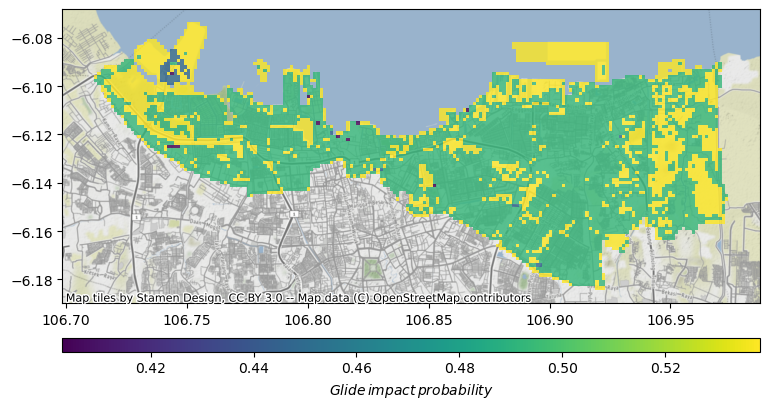
\includegraphics[width=\textwidth]{Plot/parrot/glide_pdf.png}
            \caption{Disco glide PDF}
        \end{figure}
        \begin{figure}[H]
            \centering
            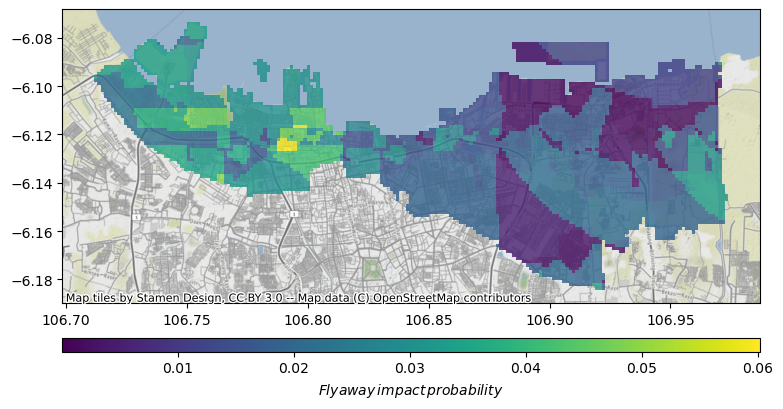
\includegraphics[width=\textwidth]{Plot/parrot/fly_away_pdf.png}
            \caption{Disco fly away PDF}
        \end{figure}
        \begin{figure}[H]
            \centering
            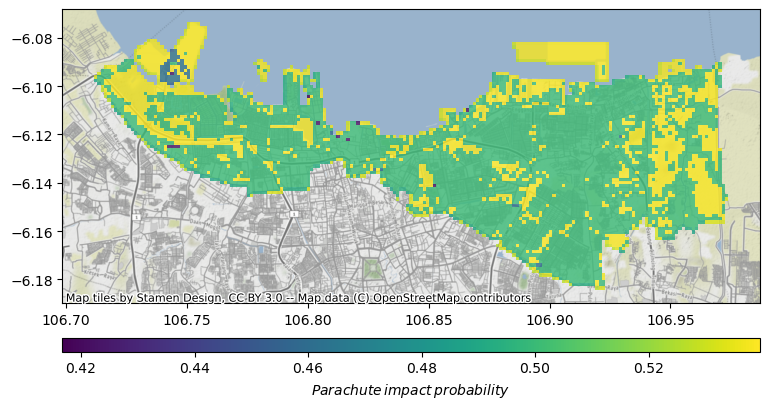
\includegraphics[width=\textwidth]{Plot/parrot/parachute_pdf.png}
            \caption{Disco parachute PDF}
        \end{figure}
        \begin{figure}[H]
            \centering
            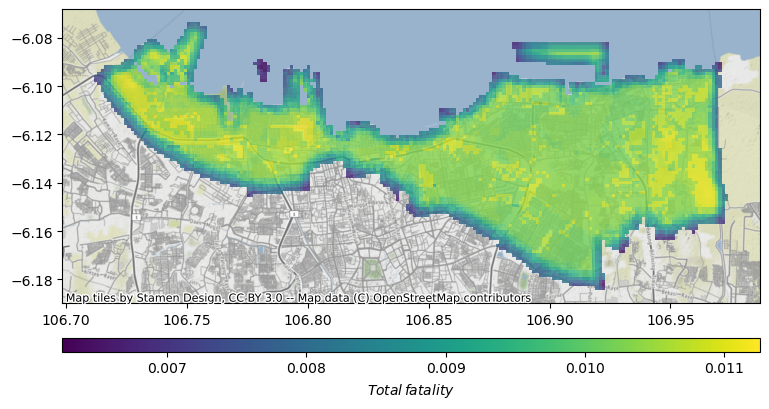
\includegraphics[width=\textwidth]{Plot/parrot/total_fatality-pdf.png}
            \caption{Disco fatality risk PDF}
        \end{figure}

        \subsection{DJI Phantom 4}
        \begin{figure}[H]
            \centering
            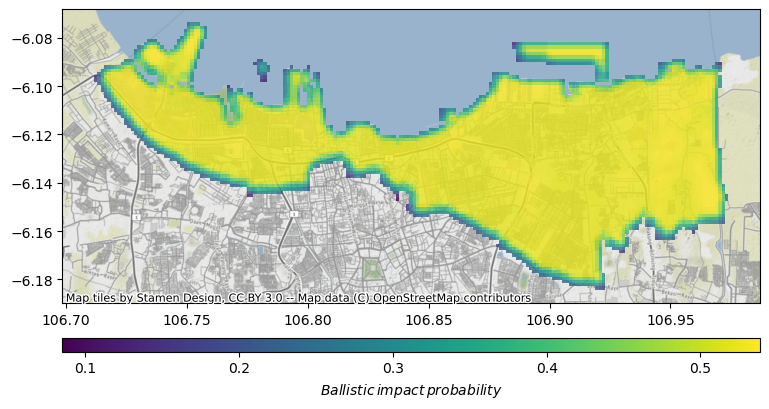
\includegraphics[width=\textwidth]{Plot/phantom4/ballistic_pdf.png}
            \caption{DJI Phantom 4 ballistic PDF}
        \end{figure}
        \begin{figure}[H]
            \centering
            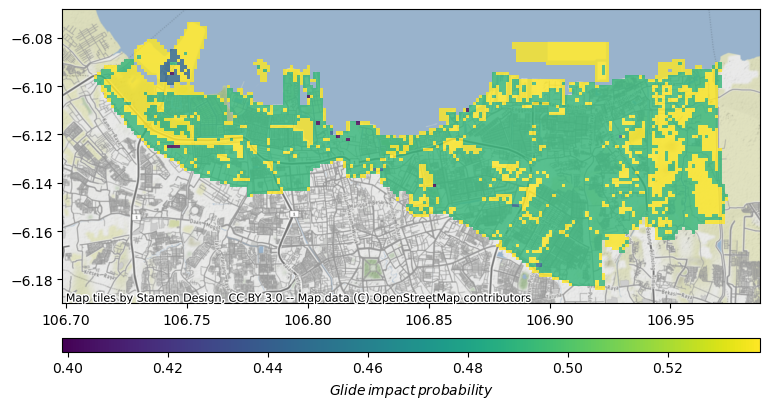
\includegraphics[width=\textwidth]{Plot/phantom4/glide_pdf.png}
            \caption{DJI Phantom 4 glide PDF}
        \end{figure}
        \begin{figure}[H]
            \centering
            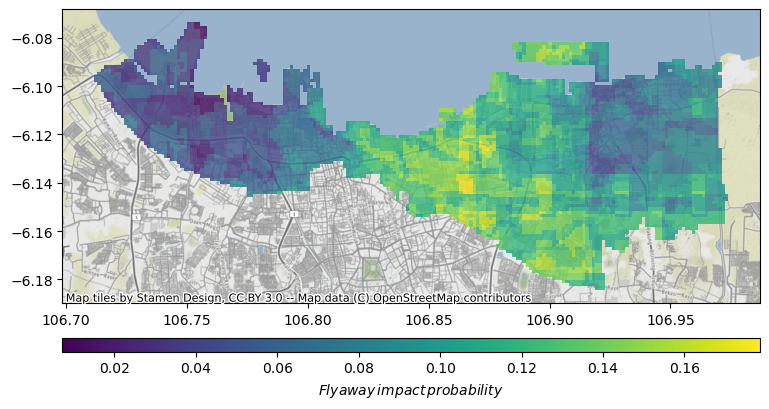
\includegraphics[width=\textwidth]{Plot/phantom4/fly_away_pdf.png}
            \caption{DJI Phantom 4 fly away PDF}
        \end{figure}
        \begin{figure}[H]
            \centering
            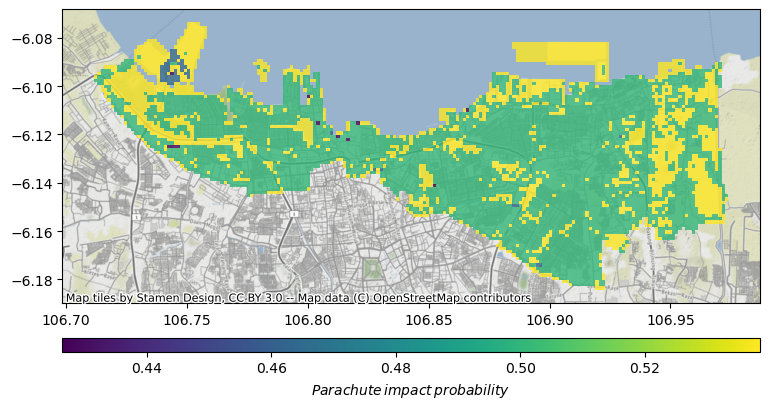
\includegraphics[width=\textwidth]{Plot/phantom4/parachute_pdf.png}
            \caption{DJI Phantom 4 parachute PDF}
        \end{figure}
        \begin{figure}[H]
            \centering
            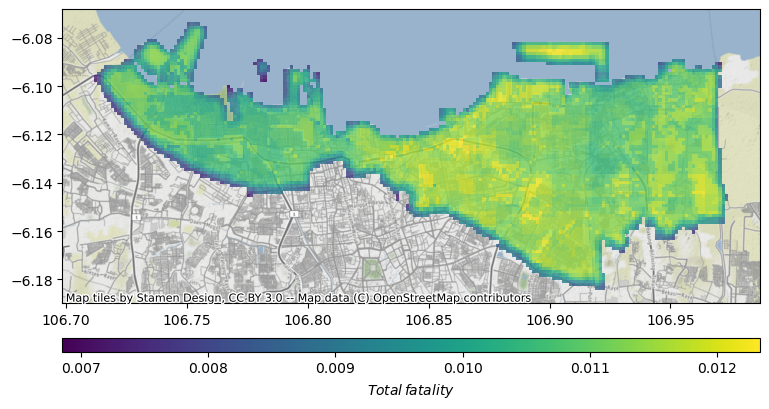
\includegraphics[width=\textwidth]{Plot/phantom4/total_fatality_pdf.png}
            \caption{DJI Phantom 4 fatality risk PDF}
        \end{figure}

        \subsection{DJI Inspire 2}
        \begin{figure}[H]
            \centering
            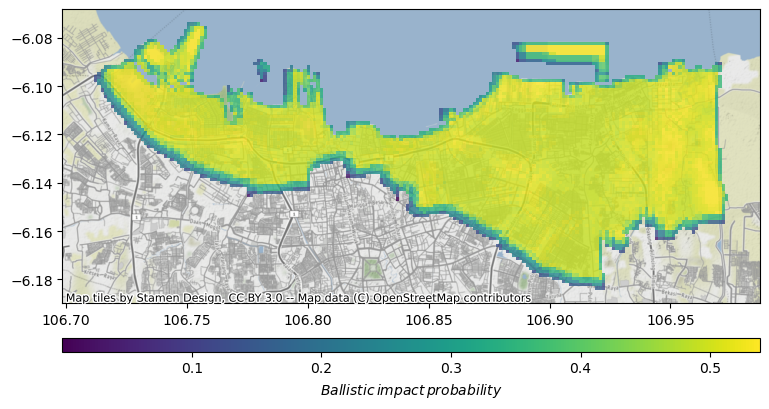
\includegraphics[width=\textwidth]{Plot/inspire/ballistic_pdf.png}
            \caption{DJI Inspire 2 ballistic PDF}
        \end{figure}
        \begin{figure}[H]
            \centering
            \includegraphics[width=\textwidth]{Plot/inspire/glide_pdf.png}
            \caption{DJI Inspire 2 glide PDF}
        \end{figure}
        \begin{figure}[H]
            \centering
            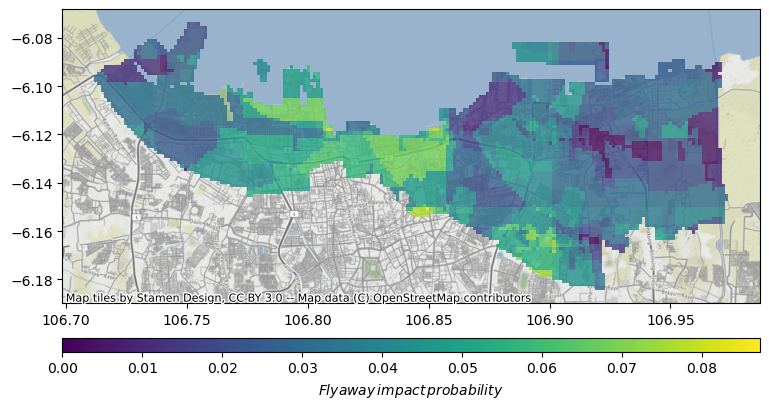
\includegraphics[width=\textwidth]{Plot/inspire/fly_away_pdf.png}
            \caption{DJI Inspire 2 fly away PDF}
        \end{figure}
        \begin{figure}[H]
            \centering
            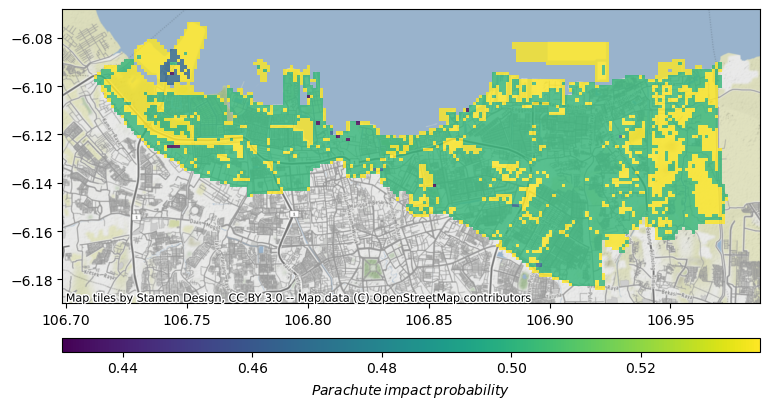
\includegraphics[width=\textwidth]{Plot/inspire/parachute_pdf.png}
            \caption{DJI Inspire 2 parachute PDF}
        \end{figure}
        \begin{figure}[H]
            \centering
            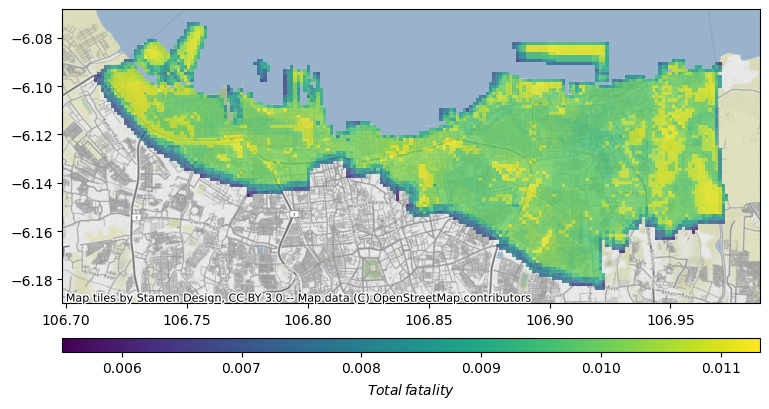
\includegraphics[width=\textwidth]{Plot/inspire/total_fatality_pdf.png}
            \caption{DJI Inspire 2 fatality risk PDF}
        \end{figure}

    \section{Pathfinder result}
        \label{fig:regularastar}
        \subsection{Regular A*}
        \begin{figure}[H]
            \centering
            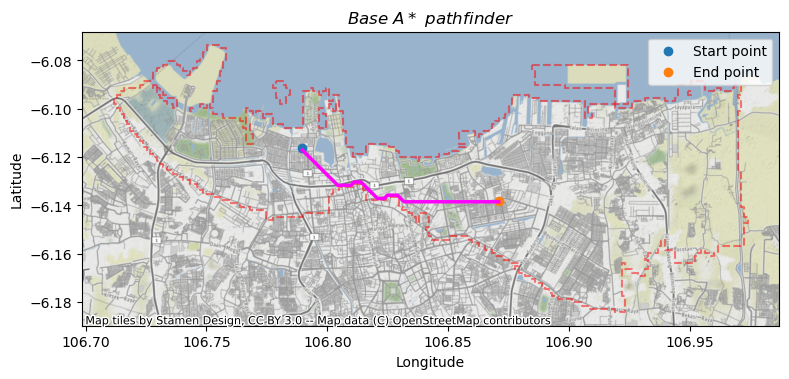
\includegraphics[width=\textwidth]{Plot/base_a_star.png}
            \caption{Regular A* flight path}
        \end{figure}

        \subsection{Risk A*}
        \begin{figure}[H]
            \centering
            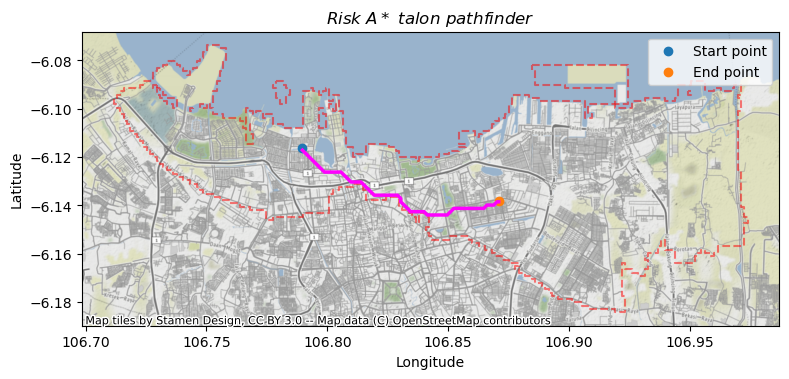
\includegraphics[width=\textwidth]{Plot/talon/talon_route.png}
            \caption{Talon risk A* flight path}
        \end{figure}
        \begin{figure}[H]
            \centering
            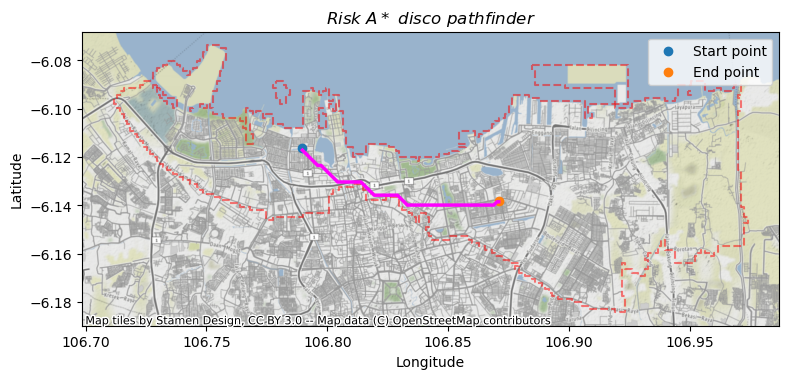
\includegraphics[width=\textwidth]{Plot/parrot/parrot_route.png}
            \caption{Disco risk A* flight path}
        \end{figure}
        \begin{figure}[H]
            \centering
            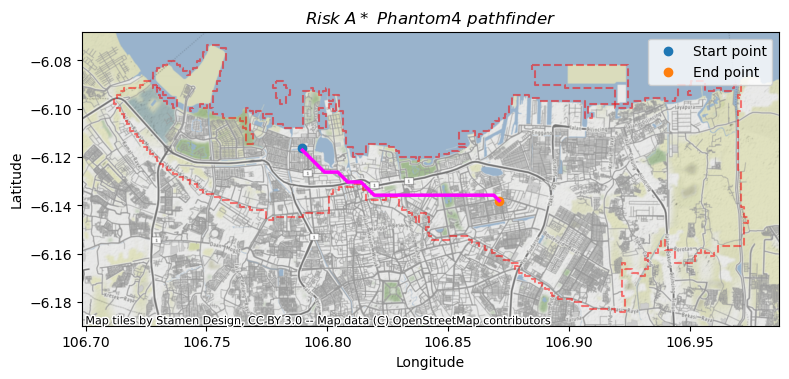
\includegraphics[width=\textwidth]{Plot/phantom4/phantom_route.png}
            \caption{DJI Phantom 4 risk A* flight path}
        \end{figure}
        \begin{figure}[H]
            \centering
            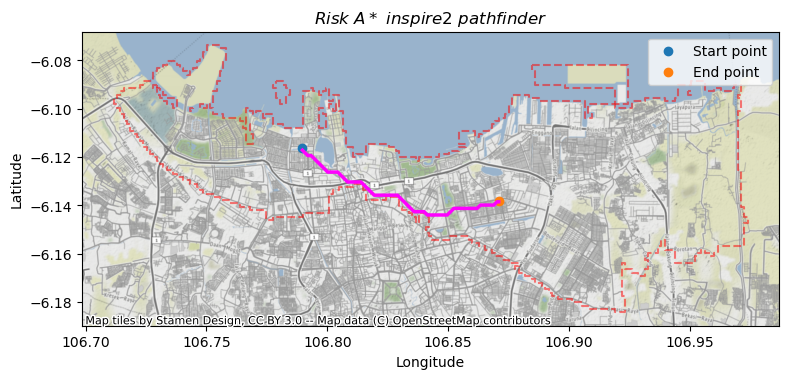
\includegraphics[width=\textwidth]{Plot/inspire/inspire_route.png}
            \caption{DJI Inspire 2 risk A* flight path}
        \end{figure}

        \subsection{Risk result}
        From \ref{fig:regularastar}, It is not surprising that the traveled distance of Normal A* is the shortest of the
        rest of the risk A*. And also, it is interesting to see that the normal A* has the highest risk, although it is
        logical to think that normal A* inversely correlates to its risk A* counterpart. It is not guaranteed for a
        normal A* to have the highest risk score. However, normal A* will guarantee to have the shortest path length
        compared to risk A*.
            
        To look at different properties, we can also measure the risk-to-traveled distance ratio, which can be thought
        of as how much the algorithm tried to avoid critical areas by extending the pathway to a much safer option. This
        example is clearly shown in DJI Phantom 4, where DJI Phantom 4 shares almost the same risk as normal A* with a
        0.02 difference, But takes a pathway that is 163 meters longer.
            
        After looking at the graph, it is tempting to use Talon since it has the lowest traveled distance and also risk
        score. However, this resulted from the limitation in the way that the program is built, which of course, needs
        some improvement.
            
        The problem lies in the Flyaway descent of this aircraft. This is because Talon has a long-range flight before
        crashing into the ground. Now the main problem is since we only use 1 cluster of geographic regions, North
        Jakarta, the region is smaller than the flyaway radius. This resulted in the outer cells of the region having a
        smaller risk compared to the center cells.
            
        It is then clear the score represented by shorter-range UAV such as Parrot Disco, DJI Phantom 4, and DJI
        Inspire 2 has a more defined score compared to the score produced by Talon.

        \begin{figure}[H]
            \centering
            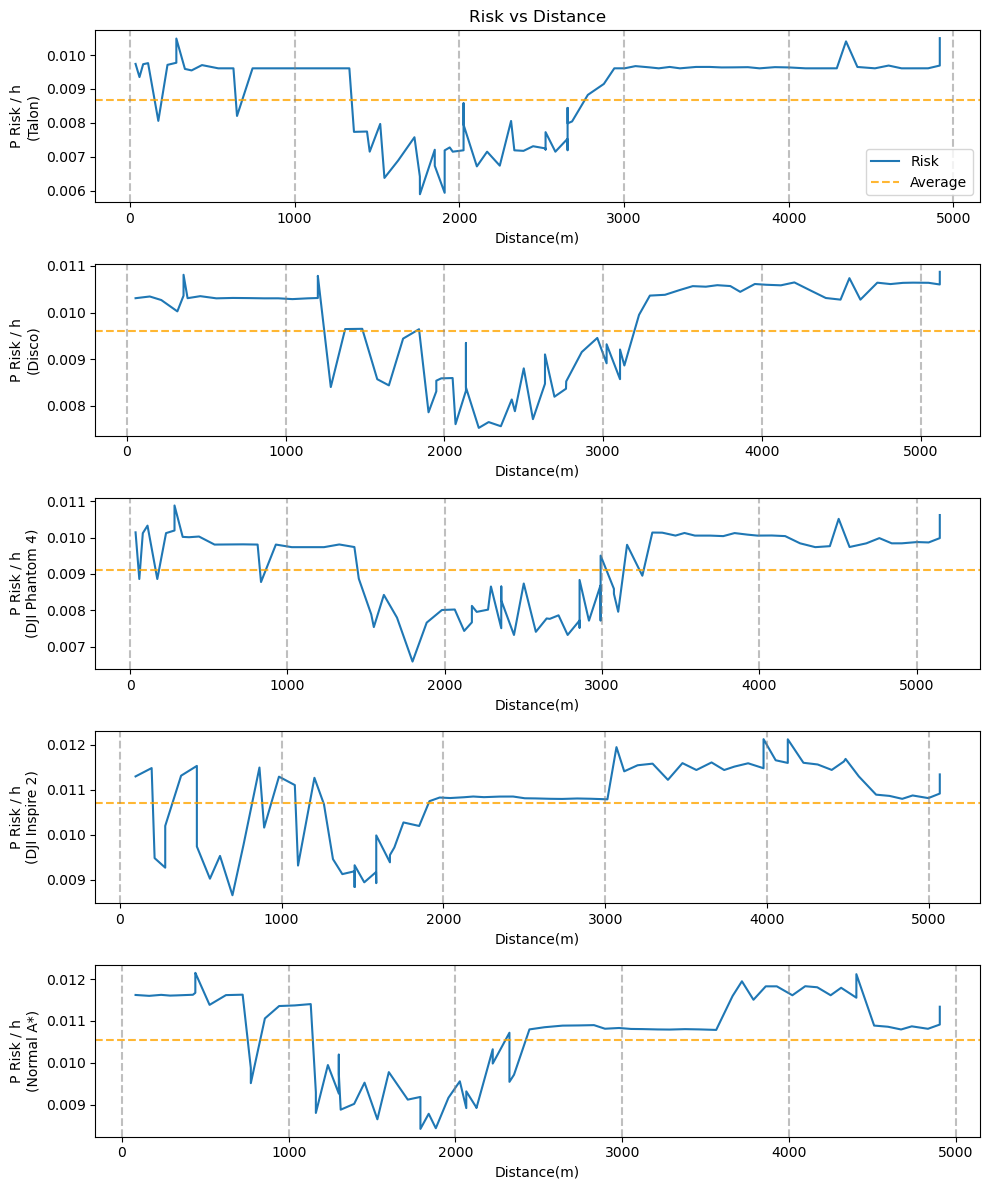
\includegraphics[width=\textwidth]{Plot/risk_vs_distance.png}
            \caption{Aircraft risk score}
        \end{figure}

        \begin{table}[H]
            \centering
            \begin{tabular}{| l  l  l  l  l |}
                \hline
                \textbf{Parameter} & \textbf{Talon} & \textbf{Disco} & \textbf{Phantom 4} & \textbf{Inspire 2} \\
                \hline
                Total travelled distance & 4917.651992 & 5120.845475 & 5066.796306 & 5147.428533 \\
                Total risk involved & 0.727661 & 0.759534 & 0.834316 & 0.765401 \\
                Risk vs distance ratio & 0.000148 & 0.000148 & 0.000165 & 0.000149 \\
                \hline
            \end{tabular}
            \caption{Total pathway risk (\%)} % Caption at the bottom
        \end{table}

    \begin{table}[H]
        \centering
        \begin{tabular}{|l l l l l l |}
            \hline
                  &  & \textbf{Ballistic} & \textbf{Glide} & \textbf{Flyaway} & \textbf{Final Risk} \\
            \textbf{Drone} &\textbf{Stat}  &  &  &  &  \\
            \hline
            \textbf{Talon} & min & 7.55e-02 & 3.14e-01 & 0.00e+00 & 5.36e-03 \\
                           & max & 5.38e-01 & 5.38e-01 & 7.76e-03 & 1.08e-02 \\
                           & avg & 4.74e-01 & 4.83e-01 & 8.47e-04 & 9.57e-03 \\
            \hline
            \textbf{Disco} & min & 5.63e-02 & 4.03e-01 & 5.38e-05 & 6.25e-03 \\
                           & max & 5.38e-01 & 5.38e-01 & 6.02e-02 & 1.13e-02 \\
                           & avg & 4.66e-01 & 5.06e-01 & 1.93e-02 & 9.91e-03 \\
            \hline
            \textbf{DJI Phantom 4} & min & 8.50e-02 & 3.99e-01 & 7.19e-03 & 6.85e-03 \\
                                    & max & 5.39e-01 & 5.38e-01 & 1.79e-01 & 1.23e-02 \\
                                    & avg & 4.87e-01 & 5.05e-01 & 9.19e-02 & 1.08e-02 \\
            \hline
            \textbf{DJI Inspire 2} & min & 6.03e-05 & 3.14e-01 & 0.00e+00 & 5.50e-03 \\
                                    & max & 5.38e-01 & 5.38e-01 & 8.72e-02 & 1.13e-02 \\
                                    & avg & 4.63e-01 & 4.83e-01 & 3.50e-02 & 9.81e-03 \\
            \hline
        \end{tabular}
        \captionsetup{justification=justified} % Caption justification
        \caption{Pathway risk statistic (\%)} % Caption at the bottom
        \label{tab:pathway-risk}
    \end{table}

    \begin{table}[H]
        \centering
        \begin{tabular}{|lllll|}
            \hline
            \textbf{} & \textbf{Talon} & \textbf{Disco} & \textbf{Phantom 4} & \textbf{Inspire 2} \\
            \hline
            {Ballistic impact probability} & 3357.142553 & 3303.336594 & 3452.695201 & 3284.220663 \\
            {Fly away impact probability} & 6.004905 & 136.521018 & 651.025645 & 248.005463 \\
            {Glide impact probability} & 3420.454716 & 3584.184491 & 3576.983890 & 3420.454716 \\
            {Parachute impact probability} & 3635.634721 & 3616.844608 & 3624.644006 & 3631.138685 \\
            {Total fatality risk probability} & 67.836022 & 69.526808 & 76.807047 & 69.526808 \\
            {Average areal total fatality risk} & 0.009572 & 0.009810 & 0.010838 & 0.009810 \\
            \hline
        \end{tabular}
        \captionsetup{justification=justified} % Caption justification
        \caption{Combine total map risk statistic (\%)} % Caption at the bottom
        \label{tab:total-map-risk}
    \end{table}


%---------------------------------------CHAPTER 5-------------------------------------
\chapter{Summary, Conclusion, and Recommendation}
    \section{Summary}
    In the summary ground, a risk map is a discrete PDF in the shape of a grid containing the possible fatality risk of
    each cell element. It is obtained by multiplying the possible outcome of multiple layers contributing to each risk.
    These layers are population density, no-fly zone layer, obstacle layer, shelter layer, and descent layer.
    \begin{myitemize}
    \item The population layer is obtained by measuring the number of people per area of the cell.
    \item The no-fly zone layer represents military and aerodrome space and its critical infrastructure that the UAV
    must not fly into
    \item The obstacle layer represents a layer where the height of the geographic features becomes an obstacle
    depending on the flight level.
    \item The shelter factor represents the capability of the building to absorb the impact energy of a crashing UAV.
    \item The descent layer is a layer that describes the probability of the drone impacting the area. The descent layer
    is split into 3 parts that additively contribute to the descent layer. These parts are ballistic descent, glide
    descent, parachute, and flyaway.        
    \end{myitemize}

    After building the ground risk map. the next step would be finding the optimal Risk A* flight path where Risk A* is
    a modified A* pathfinding algorithm, which uses risk and distance to measure the most optimal path.

    \section{Conclusion}
    Using ground risk management to measure the total area fatality of impact risk resulted in an average of:

    \begin{myitemize}
        \item Talon having $9.57 \times 10^{-3}$ fatality per flight hour
        \item Parrot Disco having $9.91 \times 10^{-3}$ fatality per flight hour
        \item Phantom 4 having $1.08 \times 10^{-2}$ fatality per flight hour
        \item Inspire 2 having $9.81 \times 10^{-3}$ fatality per flight hour
    \end{myitemize}
    With a traveled distance of each aircraft being:
    \begin{myitemize}
        \item Talon, with 4,918 m
        \item Parrot Disco, with 5,121 m
        \item Phantom 4, with 5,066 m
        \item Inspire 2, with 5,147 m
        \item Any Aircraft Without Risk involved, with 4,903 m
    \end{myitemize}
    And average path risk of aircraft:
    \begin{myitemize}
        \item Talon, with $1.48 \times 10^{-4}$ fatality per flight hour
        \item Parrot Disco, with $1.48 \times 10^{-4}$ fatality per flight hour
        \item Phantom 4, with $1.65 \times 10^{-4}$ fatality per flight hour
        \item Inspire 2, with $1.49 \times 10^{-4}$ fatality per flight hour
        \item Any Aircraft Without Risk involved, with $1.74 \times 10^{-4}$ fatality per flight hour
    \end{myitemize}

    \section{Recommendation}
        \subsection{For future research}
        \subsection{For software design}

\printbibliography
\end{document}
